\documentclass[titlepage,a4paper]{article}

\usepackage{a4wide}
\usepackage[colorlinks=true,linkcolor=black,urlcolor=blue,bookmarksopen=true]{hyperref}
\usepackage{bookmark}
\usepackage{fancyhdr}
\usepackage[spanish]{babel}
\usepackage[utf8]{inputenc}
\usepackage[T1]{fontenc}
\usepackage{graphicx}
\usepackage{float}

\usepackage{minted} %codigo

\pagestyle{fancy} % Encabezado y pie de página
\fancyhf{}
\fancyhead[L]{Apuntes sistemas operativos}
\fancyhead[R]{1C2021}
\renewcommand{\headrulewidth}{0.4pt}
\fancyfoot[C]{\thepage}
\renewcommand{\footrulewidth}{0.4pt}

\begin{document}
\begin{titlepage} % Carátula
	\hfill
\includegraphics[width=6cm]{logofiuba.jpg}
    \centering
    \vfill
    
    
\includegraphics[width=6cm]{ImagenesApunte/LogoLinux.png}
    
    \Huge \textbf{Apuntes de}
    
    \Huge \textbf{Sistemas Operativos}
    \vskip2cm
    \Large [7508] Sistemas operativos\\
    Curso Méndez \\
    1C 2021
    \vfill
    \begin{tabular}{ | l | } % Datos del alumno
      \hline
      Grassano, Bruno \\ \hline
      bgrassano@fi.uba.ar \\ \hline
  	\end{tabular}
    \vfill
    \vfill
\end{titlepage}

\tableofcontents % Índice general

\newpage

\section{Introducción}\label{sec:intro}
El presente archivo contiene los apuntes que fueron tomados a lo largo de la cursada de la materia sistemas operativos (7508) en el curso del profesor Méndez. Esta formado por parte de los mismos apuntes del curso, de anotaciones tomadas durante la clase, y en algunas partes agregue notas de la bibliografía. 

\subsection*{Recomendaciones}
Básicamente la de todas las materias, llevarla al día.

Para las teóricas conviene ir ya con el tema leído desde el \href{https://fisop.github.io/apunte/}{apunte de Mendez}, complementa también tratar de seguir las clases con alguno de los libros de la bibliografía (Sección \ref{sec:bibliografia}), personalmente fui leyendo el Arpaci, bastante claro y ordenado, los otros no tuve el tiempo de mirarlos durante la cursada.

Para las practicas, se tienen (en modalidad virtual) 2 labs que son unos trabajos prácticos individuales que se realizan al comienzo de la cursada, poniéndose un rato salen sin problemas. Dan 2 semanas para realizar cada uno.  Después de estos, sigue el TP JOS del MIT dividido en 4 partes que se realiza en grupos de a 2. Para este prepárense para dedicarle un buen tiempo, en muchos casos es poco código pero muy especifico que requiere comprender muy bien lo que se esta haciendo (me acuerdo de un caso que estuvimos mas de una hora para hacer 2 lineas de código). Para cada parte lean bien las diferentes consignas, ya que aportan diferentes datos (la del curso, la original del MIT, y la del código).

\newpage

\section*{Primera clase}
\section{¿Que es un sistema operativo?}

Es la capa de software que maneja los recursos de una computadora para sus usuarios y sus aplicaciones. Normalmente estos son invisibles a los ojos del usuario. (\textit{Auto, Avión, Cámara, etc})

En un sistema operativo de propósito general, los usuarios interactúan con aplicaciones, estas aplicaciones se ejecutan en un ambiente que es proporcionado por el sistema operativo. A su vez el sistema operativo hace de mediador para tener acceso al hardware del equipo.

La principal forma para lograr esto es mediante el concepto de \textbf{virtualización}. Esto significa que el sistema operativo toma un recurso físico (\textit{Ej. Memorias, procesadores, persistencia}) y lo transforma en algo mas general y fácil de usar.

\subsection*{Roles del OS}

\begin{itemize}
    \item \textbf{Referee}: El sistema operativo gestiona recursos compartidos entre diferentes aplicaciones. Estos están ejecutándose en la misma maquina física. \textit{Acciones posibles: Frenar aplicaciones e iniciar otra, aislar aplicaciones de recursos, decidir que aplicación usa que recurso.}
    \item \textbf{Ilusionista}: Provee la ilusión de que se dispone de toda la memoria para almacenar el programa, cuando realmente la memoria principal es finita. Da la abstracción del hardware para simplificar el diseño de los programas.
    \item \textbf{Pegamento}: Debe proveer una serie de servicios comunes que faciliten un mecanismo para compartir, una API, un conjunto de funciones que parezcan que están diseñadas con el mismo criterio. \textit{Ej. accesos a entrada/salida, ctrl+c/ctrl+v de manera uniforme a lo largo del sistema}
\end{itemize}

\begin{figure}[!htb]
    \centering
    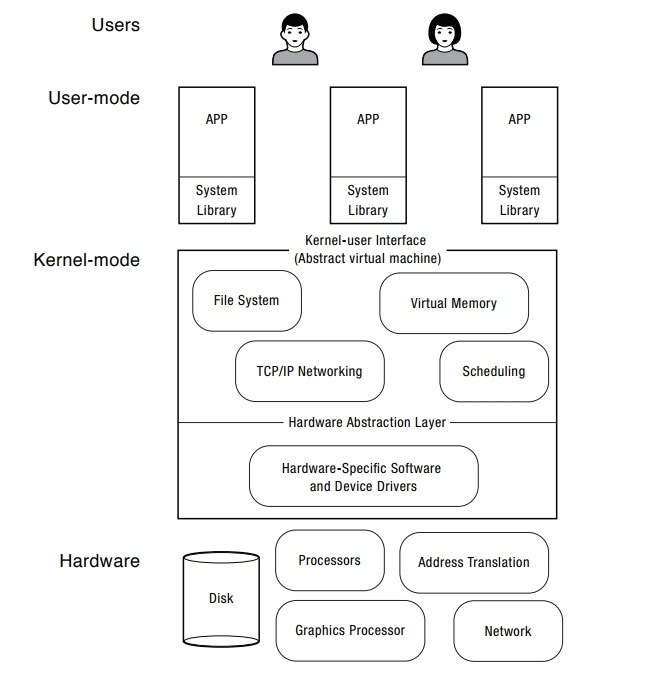
\includegraphics[width=0.7\textwidth]{ImagenesApunte/SystemaOperativoCapas.jpg}
\end{figure}


\subsection*{Modos de ejecución}

Existen dos modos de ejecución.
\begin{itemize}
    \item El sistema operativo se ejecuta como la capa \textbf{de software} de mas bajo nivel en la computadora. Este contiene una capa para la gestión de dispositivos, y por otro lado una serie de servicios para la gestión de dispositivos agnósticos del hardware. Estas capas son conocidas como el \textbf{kernel} del sistema operativo. Si parte del código fuente de esta capa es ejecutado, la computadora pasa a un estado llamado \textbf{Modo Supervisor}. Estas capas pueden utilizar primitivas que provee el hardware para el aislamiento de fallas y sincronización. El termino de kernel puede ser equivalente al de sistema operativo. Gracias a la existencia del kernel, los programas son independientes del hardware subyacente. Tener en cuenta que el kernel es un programa. No confundir esto con el modo \textit{root} de linux ni correr con privilegios.
    
    \item Las aplicaciones mientras tanto, se ejecutan en un contexto \textbf{aislado, protegido y restringido}. Este contexto de ejecución se llama \textbf{User Mode} y mediante funciones de bibliotecas pueden utilizar los servicios de acceso al hardware o recursos que el kernel proporciona.

\end{itemize}

\subsection*{Perspectiva del usuario}

El usuario lo que puede 'ver' son tres partes: el sistema de archivos, el entorno de procesamiento, y los bloques primitivos de construcción.

\subsubsection*{Sistema de archivos}

En UNIX es una estructura jerárquica que permite el tratamiento consistente entre diferentes archivos. Permite crear, borrar, proteger o modificar archivos (que crezcan en tamaño de forma dinámica).
Esta organizado como un árbol con una una raíz (/). Cada nodo no hoja del sistema de archivos se denomina directorio de archivos, y las hojas del árbol pueden ser a su vez archivos, directorios, o archivos especiales. Cada uno de estos tiene un nombre dado por el camino (path) para localizarlo en la estructura.

\subsubsection*{Entorno de procesamiento}
Un programa es un archivo ejecutable. Un proceso es una instancia de un programa en ejecución. Cada programa puede tener muchos procesos ejecutándose a la vez, no hay un limite lógico para la cantidad.

El primer programa en ser ejecutado es el interprete de comandos (shell) en UNIX en modo usuario (no es parte del kernel del sistema operativo). Este una vez cargado ejecuta el comando \textit{login}.

\subsubsection*{Bloques primitivos de construcción}
La idea de UNIX es la de proveer mecanismos para que los programadores construyan programas complejos a partir de programas mas pequeños. \textit{Divide y conquista}

\subsection*{El proceso}
El proceso es la parte fundamental de cualquier sistema operativo. Es una abstracción. Un programa en ejecución. El programa almacenado en disco contiene el código fuente compilado y los datos del mismo. A partir de estos los sistemas operativos permiten darle vida a los ejecutables, convirtiéndose en un proceso. Se puede ver como el espacio de memoria donde se aloja el programa que esta siendo ejecutado.

% fork diferencia de valor de retorno es lo que hace que tomen otro camino - funcion que devuelve dos cosas diferentes en diferentes procesos - revisar documentacion - man fork -> FORK(2) el 2 es del capitulo de syscalls - retorno < 0 fallo fork - si es 0 es el hijo - en el padre devuelve el valor del hijo - direcciones virtuales estan aisladas entre si - no falla con archivos, tiene la misma referencia, el archivo es uno solo (el file descriptor es accesible desde ambos procesos - si cierro en uno, tengo que cerrar el otro file descriptor) - los procesos se comunican con pipe() los procesos lo ven como file descriptor, es como un archivo virtual, el pipe es unidireccional, la lectura bloquea hasta que haya algo que leer, el OS lo guarda hasta que alguien lo quiera leer - con un pipe podemos garantizar cierto orden - Unix: A History and a Memoir - pipe(int pipefd[2]) primero extremo lectura, el segundo es de escritura, contienen el file descriptor - importante cerrar el extremo que no vamos a usar - para usarlo bidireccionalmente hay que usar 2 pipes (forma mas correcta) - revisar que write devuelva el tamaño de lo que escribimos, tambien en read, read hace el intento de leer - encerrar el write  while(bytes_leidos < bytes_a_leer){...} - ambos proceso tienen que estar de a cuerdo en el tamaño que se lle

% LAB FORK pingpong: 2 pipes, bidireccional, syscalls, getpid, getppid
% primes: generar procesos on demand, tantos procesos como primos haya entre 0 y n, generador que hace todos los numeros de 2 a n, NO almacenarlos todos en memoria, ir generandolos, 2*n, 3*n,5*n,...los numeros que no descarta un filtro se los pasa al siguiente, sigue hasta que quede un solo primo, una vez llegado ahi tiene que cerrar todo, tienen que ser creados iterativamente los filtros, cuando me doy cuenta que necesito uno ma - la logica del filtro sabe crear un filtro nuevo si lo necesita - en 2 semanas la entrega de los 4 ejs del lab


\section*{Segunda clase}


\section{El Kernel} % GNU Linux = kernel + apps ----- Linux = kernel ---- OS en la materia = kernel --- afuera OS = kernel + apps

\subsection*{Ejecución directa}
La ejecución directa consiste en correr el programa directamente en la CPU. Esto otorga la ventaja de tener rapidez. Aunque también esto viene con algunos problemas. Estos son: ¿Como se asegura el OS que el programa no va a hacer nada que el usuario no quiere que sea hecho? ¿Como hace el OS para pausar la ejecución de ese programa y hacer que se ejecute otro?

Debido a esto se necesita limitar la ejecución directa. Hoy en día esto ya no existe en un sistema operativo serio.

\subsection*{Limitar la ejecución directa}

Para poder limitar la ejecución directa, son necesarios mecanismos del hardware.

\begin{itemize}
    \item Dual Mode Operation - Modo de operación dual
    \item Privileged Instructions - Instrucciones Privilegiadas
    \item Memory Protection - Protección de Memoria
    \item Timer Interrupts - Interrupciones por temporizador
\end{itemize}

\subsubsection*{Dual Mode Operation}
En las arquitecturas de x86 se tienen 4 modos de operaciones vía el hardware. Van del 0 a 3 y se denominan \textbf{rings}, siendo el ring 0 el nivel mas privilegiado (el del kernel - modo supervisor o modo kernel) y el 3 el menos (el de las aplicaciones - modo usuario). El hardware chequea en que modo de operación se esta ejecutando cada instrucción. La diferencia entre ambos modos esta en un bit en el registro de control del procesador. Tener esto permite proteger la memoria, los puertos de I/O y la posibilidad de ejecutar ciertas instrucciones.


\begin{figure}[!htb]
    \centering
    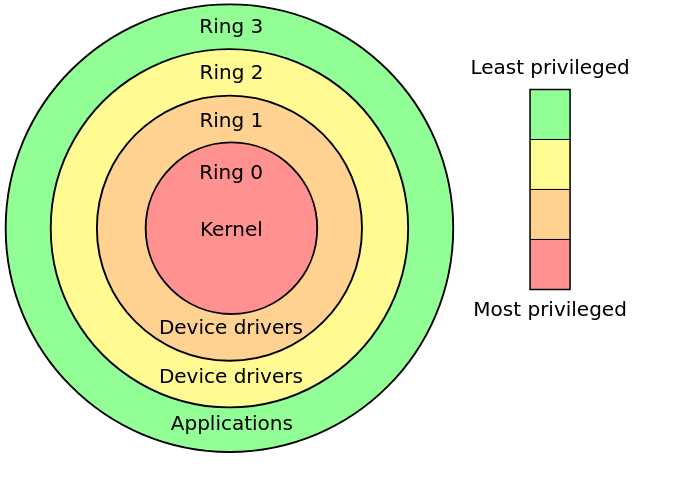
\includegraphics[width=0.7\textwidth]{ImagenesApunte/rings.png}
\end{figure}


\subsubsection*{Protección del sistema}

\begin{itemize}
    \item Que se tenga el modo dual permite que cada modo tenga su propio set de instrucciones. Con lo cual el bit de modo de operación indica al procesador si la instrucción ejecutada puede ser o no ejecutada, según el modo en que se encuentre. (Instrucciones privilegiadas) \textit{Un ejemplo de estas instrucciones es LGDT}
    
    \item En el caso de la protección de la memoria, el sistema operativo debe poder configurar el hardware de forma tal de que cada proceso pueda leer y escribir su propia porción de memoria, ya que ambos, sistema y aplicaciones están en memoria al mismo tiempo.
\end{itemize}


\subsubsection*{Timer Interrupts}

Cuando se ejecuta una aplicación, esta cree que tiene todo el tiempo para realizar lo que quiera, pero en realidad es una ilusión. El hardware proporciona al kernel un \textbf{hardware counter}, el cual una vez seteado, interrumpe el procesador luego de un determinado tiempo. Esto permite que el kernel desaloje el proceso del usuario y tome el control de la maquina. 

El programa no se da cuenta que se despierta el kernel.

Con este sistema no hay forma de que un programa se quede con todo el procesamiento, ya que vuelve al kernel despues de un tiempo. 

\subsection*{IOPL}
El IOPL son los bits que se agregaron para poder identificar en que modo (ring) se esta. Se puede cambiar de privilegio con unas funciones, las cuales solo pueden se usadas desde el modo kernel (POPF(D)). Son los bits 12 y 13 del registro de flags.

\begin{figure}[!htb]
    \centering
    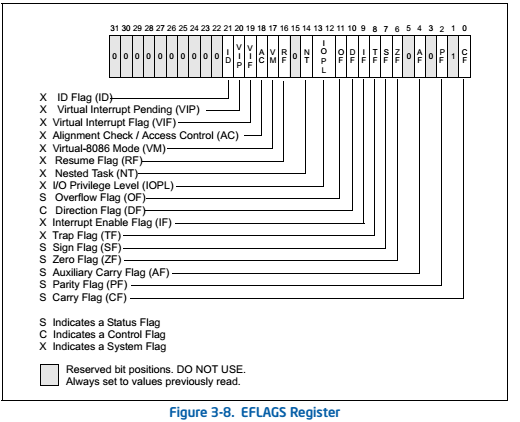
\includegraphics[width=0.7\textwidth]{ImagenesApunte/FlagsRegister.png}
    \caption{Bits del registro de flags}
\end{figure}

\subsection*{Tareas del kernel}

\begin{itemize}
    \item Planificar la ejecución de las aplicaciones, toda aplicación que se ejecuta, la planifica el kernel. Hay un modulo especifico para esto, el scheduler. \textit{El famoso Árbol rojo negro}.
    \item Gestionar la Memoria, asignar el recurso, decir quien puede y quien no usarla. También el como puede usarla.
    \item Proveer un sistema de archivos
    \item Creación y finalización de procesos
    \item Acceder a los dispositivos
    \item Comunicaciones
    \item Proveer un API para acceder al hardware
\end{itemize}

\subsection*{Transferencias}
Existen tres formas para cambiar de modo usuario a modo kernel: con interrupciones (evento externo), con excepciones del procesador ()evento interno, y mediante la ejecución de \textit{system calls} (evento intencional). (6 en total, de usuario a kernel, y de kernel a usuario)

\subsubsection*{Interrupciones}

Una interrupción es una señal asincrónica enviada hacia el procesador que indica que algún evento externo ha sucedido, causando que se pueda requerir de la atención del mismo. El CPU esta revisando continuamente si se dispara alguna interrupción. Si sucede alguna, completa o detiene cualquier instrucción que se este ejecutando, y en vez de ejecutar la siguiente instrucción, guarda el contexto, y comienza la ejecución del manejador de esa interrupción en el kernel.

Es externo al procesador.

\subsubsection*{Excepciones del procesador}

Estas excepciones son causadas por el programa de un usuario. Sigue el mismo funcionamiento que el de una interrupción. \textit{Ej. Acceder fuera de la memoria del proceso, intentar ejecutar una instrucción privilegiada en modo usuario, intentar escribir en memoria de solo lectura, dividir por cero}.

\subsubsection*{System Calls}

Las System Calls son funciones que permiten a los procesos del usuario pedirle al kernel que realice operaciones en su nombre (puntos de entrada controlados al kernel). Las system calls conforman una API.

El uso de estas llamadas cambia el modo del procesador de \textit{user mode} a \textit{kernel mode}. El conjunto que se ofrece de opciones es fijo. Cada system call esta identificada por un numero fijo que no es visible al programa, solamente se conoce su nombre.

La llamada a una system call es similar a la invocación a una función de C, aunque detrás hay varias diferencias. La función que se ve en C actúa como un \textit{wrapper} (envoltorio). Esta función que envuelve a la system call proporciona todos los argumentos al \textbf{system call trap\_handling}, los cuales son pasados por el stack (hay casos en que los espera en determinados registros, ahí son copiados por el wrapper también).

Al momento de ejecutarse, las system calls son identificadas por el kernel con un numero en un registro (\%eax) y se ejecuta una instrucción de código maquina llamada \textbf{trap machine instruction} (0x80) (una interrupción) que causa el cambio a \textit{kernel mode} y se ejecute el código del vector de traps el sistema. En respuesta a esto el kernel invoca a su propia función para manejar esa trap finalmente. Si se devuelve error, la función wrapper lo setea en \textit{errno}.

Las syscalls son llamadas desde el modo usuario. (con el wrapper). 

\begin{figure}[!htb]
    \centering
    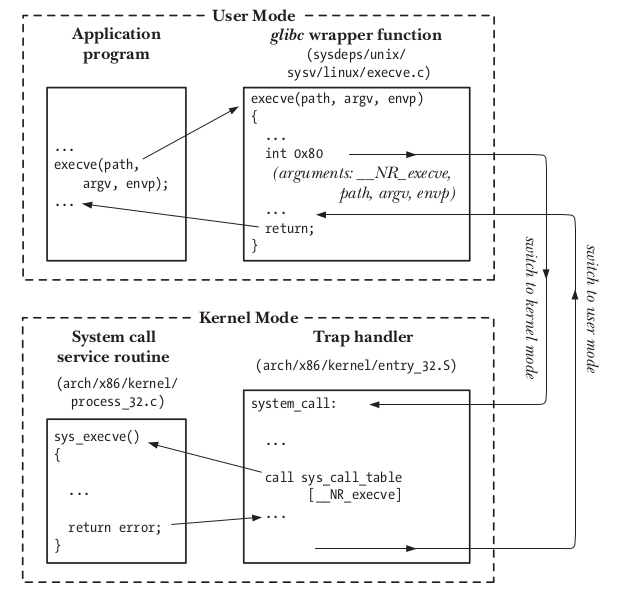
\includegraphics[width=0.7\textwidth]{ImagenesApunte/system_calls.png}
\end{figure}

\subsection*{De Kernel a  usuario}
\begin{itemize}
    \item Crear un nuevo proceso.
    \item Continuar después de una interrupción, excepción o system call. Una vez que el kernel manejo el pedido, continua con el proceso interrumpido. (cambiando a modo usuario)
    \item Cambio entre procesos, se ejecuta un proceso, salta la interrupción, cambio a otro debido a que el otro se estaba ejecutando mucho.
\end{itemize}

\subsection*{Linux}

Linux no es un sistema operativo, es solo un kernel (Desarrollado por Linus). El resto de los componentes están hechos por terceros. \textit{Ej. GNU}. Algunas características de este kernel son:

\begin{itemize}
    \item No tiene acceso a la biblioteca estándar de C, ni a los encabezados.
    \item Esta codificado con GNU C.
    \item El kernel no se protege de si mismo.
    \item No puede realizar fácilmente operaciones de punto flotante.
    \item El kernel tiene una pila fija de tamaño pequeño, no es dinámica.
    \item Es un único programa ejecutándose en memoria. (Kernel monolítico)
    \item El kernel tiene interrupciones sincrónicas, es preentive (el kernel te desaloja) y admite SMP.
\end{itemize}


\subsection*{Tipos de kernel}
\begin{itemize}
    \item Kernel Monolítico: es un programa único (proceso) que se ejecuta continuamente en memoria intercambiándose con los procesos del usuario. \textit{Ej. Linux}
    \item Micro Kernel: solo implementa funcionalidad básica (en Ring 0). ~4000 lineas de código. \textit{Ej. MINIX}
\end{itemize}

\subsection*{Inicio}
El proceso de inicio comienza con el booteo, denominado bootstrap. Esta parte depende del hardware, ya que acá se realizan chequeos del mismo y se carga el bootloadler, que es el encargado de cargar el kernel del sistema operativo. Esto se divide en 3 partes.
\begin{enumerate}
    \item Se carga el BIOS (Basic Input/Output System)
    \item Se crea la Interrupt Vector Table, y carga las rutinas de manejo de interrupciones en Modo Real.
    \item El BIOS genera una interrupción (19), la cual hace ejecutar el servicio de interrupciones.
\end{enumerate}

Luego del booteo, el BootLoader pasa a modo supervisor (posible por ser vía hardware), busca el kernel en el dispositivo de almacenamiento correspondiente y lo carga a memoria principal (esta como un archivo imagen, comprimido). Una vez hecho eso, setea el registro de la próxima instrucción y ejecuta la primer linea del kernel.

Una vez cargado y ejecutado el kernel, se cargan a memoria las aplicaciones que se deben ejecutar (shell), se setea la siguiente instrucción, y se pasa a modo usuario, dándole control a la aplicación.

\subsection*{Fase de inicio}
La función de arranque para el kernel (intercambiador o proceso 0) establece la gestión de memoria (tablas de paginación y de memoria), detecta el tipo de CPU, funcionalidades adicionales (\textit{ej. punto flotante}), y después cambia a funcionalidades del kernel no especificas de Linux a través de \textit{start\_kernel()}.

Esta función establece el manejo de interrupciones, configura memoria adicional, y comienza el proceso de inicialización. El primer proceso ejecutado por el sistema es \textit{Init} (PID = 1).

El proceso Init se encarga de comprobar y montar los sistemas de archivos y poner en marcha los servicios de usuario necesarios y, en última instancia, cambiar al entorno de usuario cuando el inicio del sistema se ha completado.


%crear rama base_fork (estado comun), subir a entrega_fork(lab_fork), agregar .gitignore para sacar los *.o, ide -> echo "*.o" > .gitignore
%agregar cerrado de pipe linea 107, else linea 126 sacarle el if() mover el else arriba
%wait hace que el proceso no utilice recursos del cpu, de forma similar a sleep, solo que el os te pone a dormir y espera a otro proceso, de padre a hijo
%ctrl+z en terminal, pone el proceso a dormir :O

%agregar if en el wait, resultado del wait tambien
%archivo de texto explicando primes, que mecanismo usamos
%no usar printf, cambiar a write file descriptor 1 (stdout) - probar mandando a archivo

%lab fork2
%find
%todo la data esta encodeada en el directorio, el que sabe como se llaman los archivos es el directorio, alcanza con abrir directorios y ver la lista de entradas que tienen - el archivo en si lo unico que tiene son los contenidos, no se como se llama ni donde esta parado
%opendir(3) y readdir(3), no leen el binario, nos dan una estructura amigable para operar mejor. No son syscalls, usan estructuras DIR* y structr dirent*, llamadas consecutivas devuelven las siguientes (punteros a directorios), al final devuelve NULL - nos imporatn d_type = DT_DIR y DT_REG
% DIR PADRE: .. - DIR PROPIO: . - La lista tiene estas dos entradas tambien - CUIDADO CON LA RECURSIVIDAD!!!!!!!!!!!!!!!!!!!!!!!!!! filtrar o ignorar esos directorios especiales
% tener en cuenta que pueden fallar

% a opendir(3) hay que pasarle el path completo -> concatenar cadenas,feo -> recomendable: openat(2) da un fd que es como un open regular pero relativo, el fd representa ese subdirectorio abierto, se facilita recorrer recursivamente el arbol de archivos, como converto de dir a fd? dirfd(3) y fdopendir(3) para convertir de los 2 formatos.
% strstr(3) y strcasestr(3) devuelven un punto de la cadena, si existe ya esta para nosotros. buscan la primer ocurrencia de la 'aguja'

%xargs
%herramienta para ejecutar un programa repetidas veces sobre varios inputs, 
%ls esta en /bin, los comandos estan aca $PATH
%xargs crea un nuevo proceso y le da una identidad distinta, usamos fork(2) y execve(2), execve no crea procesos nuevos, lo que hace es cambiar identidad - la shell hace fork y despues execve para correr un binario distinto - cambia la iumagen de un proceso, memoria virtual, entorno, argumentos, pero mantiene fd, pid,ppid, etc - esta syscall es unica

%familia exec(3) - execvp para facilitar la busqueda de binarios en path - se recomienta execvp - son wrappers que llaman a la unica syscall execve(2) notar la parte del manual (2 - 3)
%no existe un return de un exec, muere el proceso viejo, termina directamente - verificar los casos de error, pasarle null, no existe binario, la ejecucion continua
%investigar dup(2)

% -n NARGS - de a cuantos argumentos lee para cada ejecucion, si es >1 los argumentos se pasan, remover \n al final - usar wait para que se ejecuten secuencialmente (no lanzar la segunda ejecucion hasta que termine la primera)

%extra: flag adicional -P, hasta 4 ejecuciones corriendo en paralelo, es usar un poco mas los waits

%entrega viernes a la noche - para cambios finales se puede hasta el domingo 2/5

\newpage

\section*{Tercera y cuarta clase}

\section{Introducción x86}

\subsection*{Ley de Moore}
En el 1965 Gordon Moore formulo la ley empírica que se ha podido constatar hasta hoy en día. Esta dice:
\textit{'Aproximadamente cada dos años se duplica el número de transistores en un microprocesador por unidad de área'}.

\begin{figure}[!htb]
    \centering
    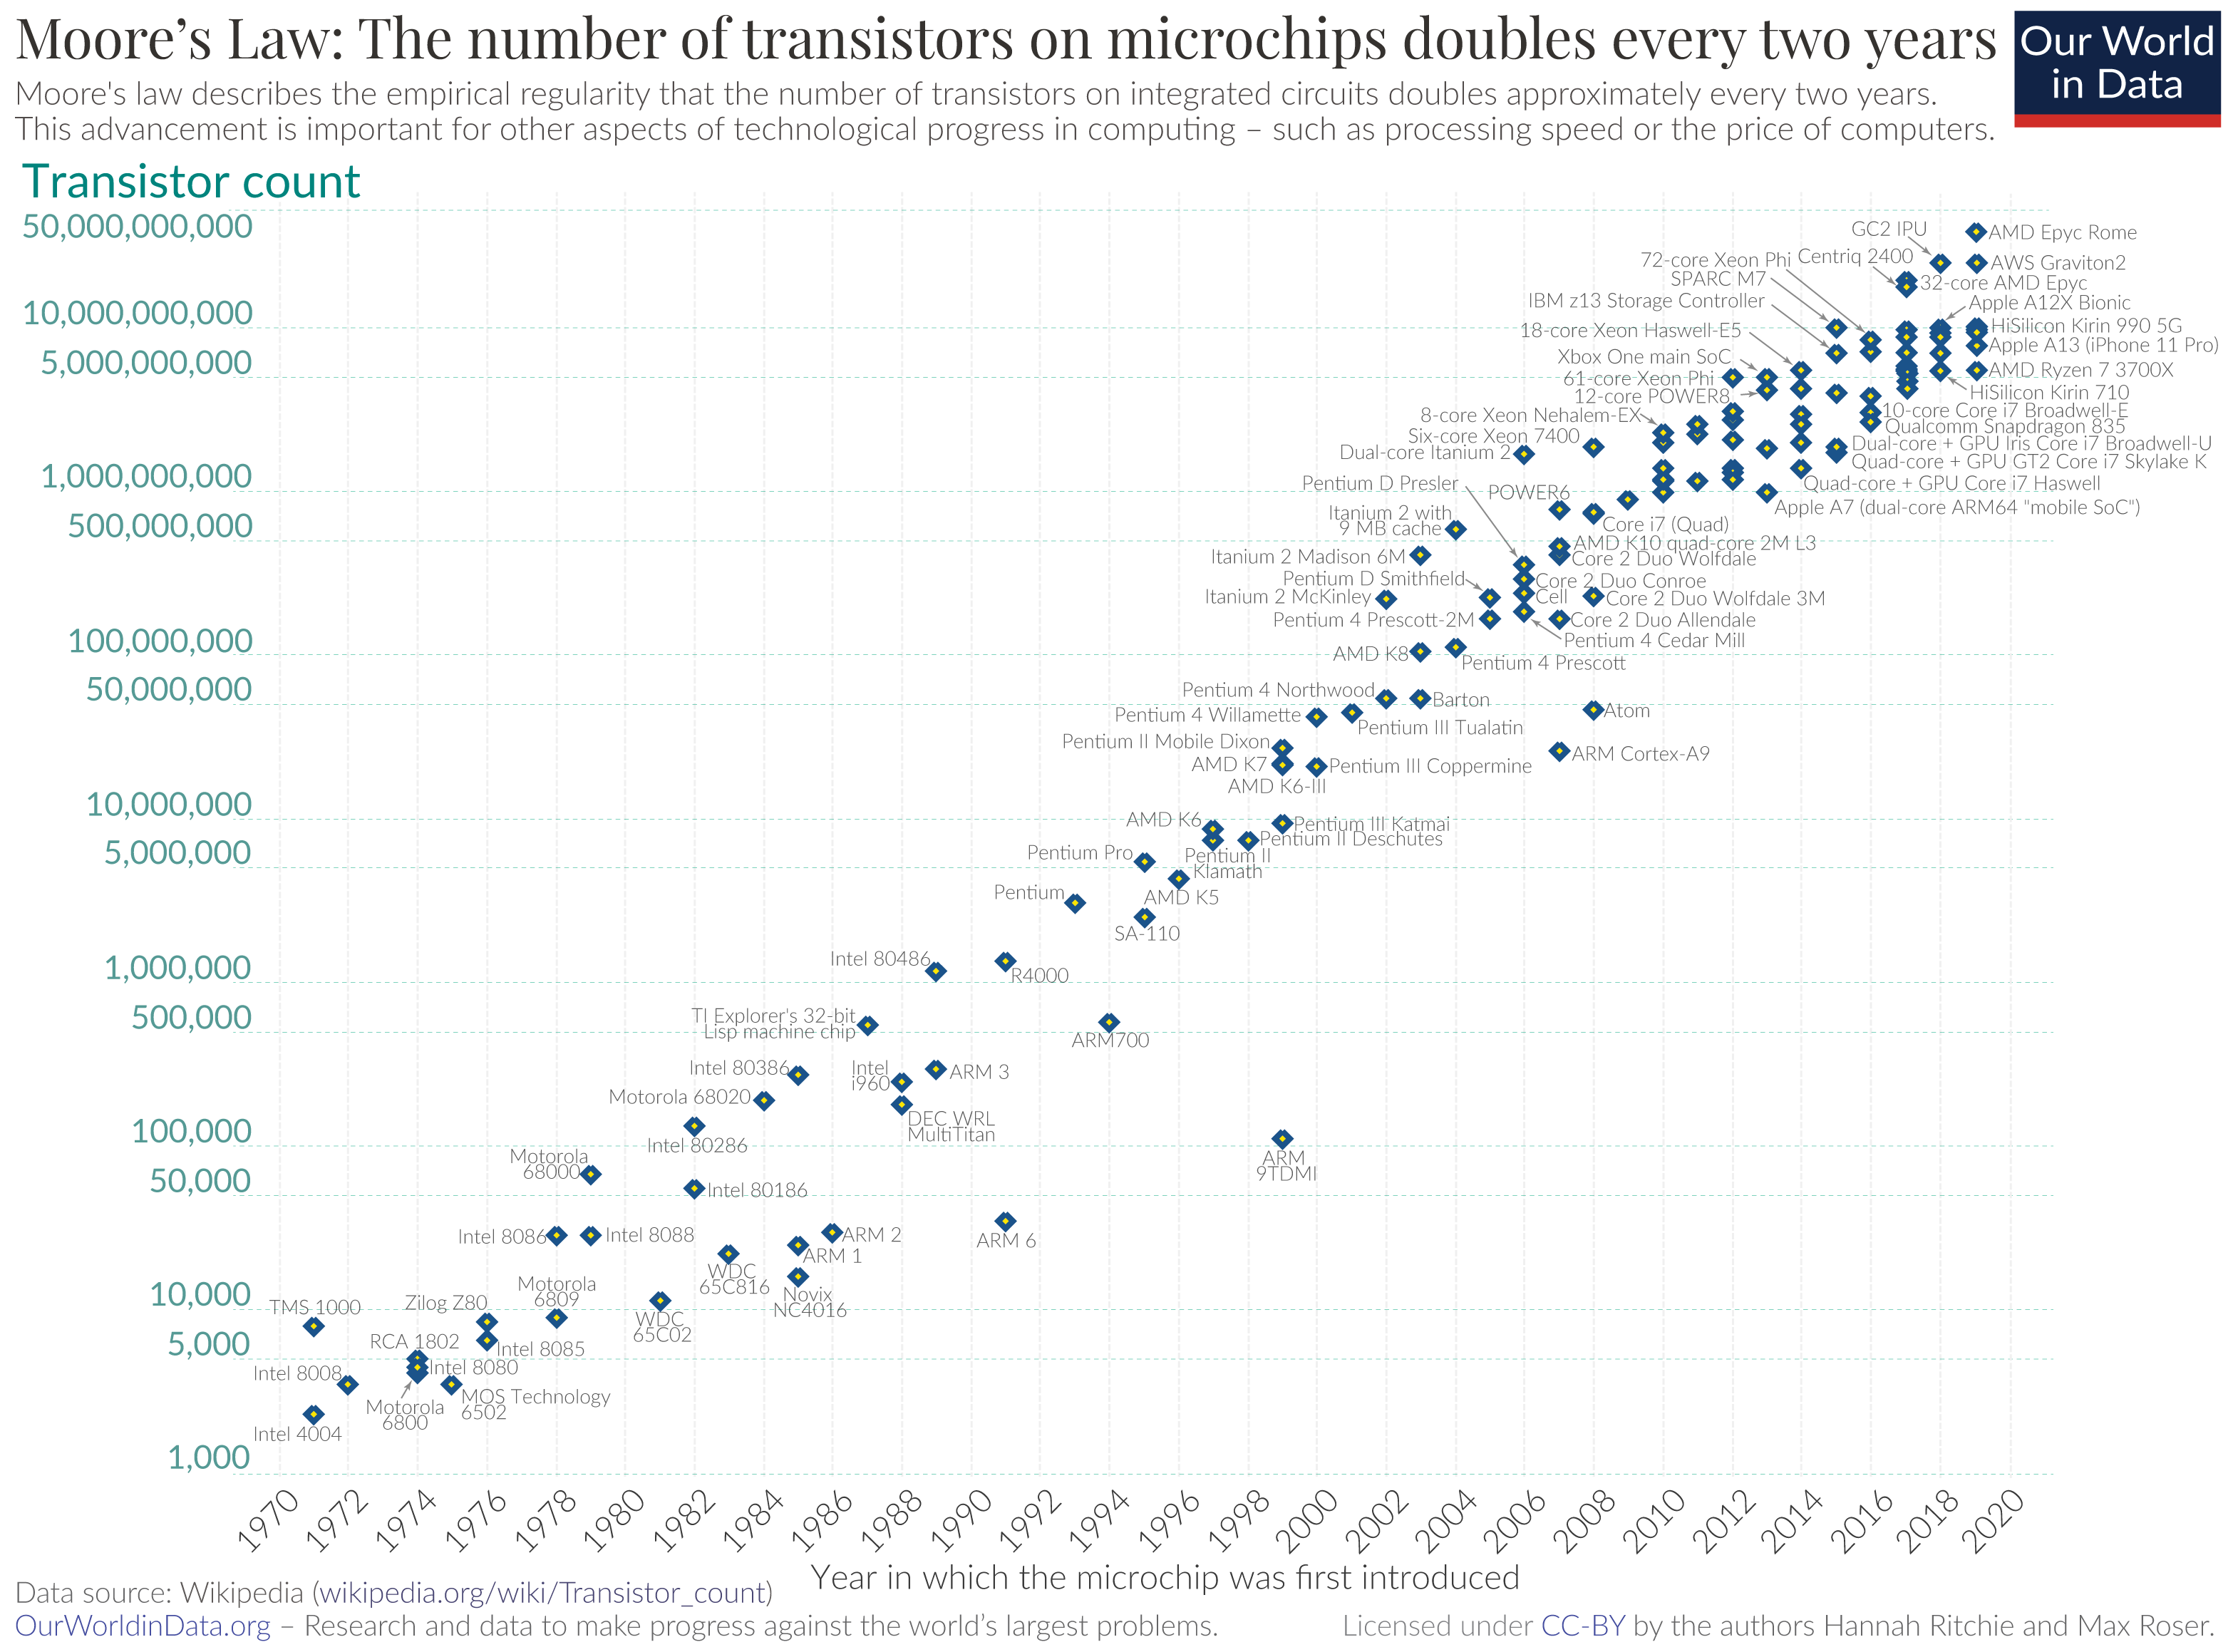
\includegraphics[width=0.9\textwidth]{ImagenesApunte/MooresLaw.png}
    \caption{Evolución de la cantidad de transistores.}
\end{figure}


\subsection*{Ley de Bell}
Esta ley establece que aproximadamente cada diez años una forma nueva de computadoras basadas en una nueva forma de programación, networking e interface se establece como nuevo uso de la industria.


\subsection*{Arquitectura x86: Hardware}
El primer modelo de programación se denomino \textit{program visible} debido a que sus registros utilizados durante la ejecución del programa y son especificados por las instrucciones. \textit{Ej. ADD dx,cs}

Existe otros tipos de registros que son \textit{program invisible} ya que no son direccionables directamente en tiempo de ejecución del programa. Únicamente a partir del 80286 existen registros program-invisible, utilizados exclusivamente para control y para operar con memoria protegida, entre otras cosas.

\begin{figure}[!htb]
    \centering
    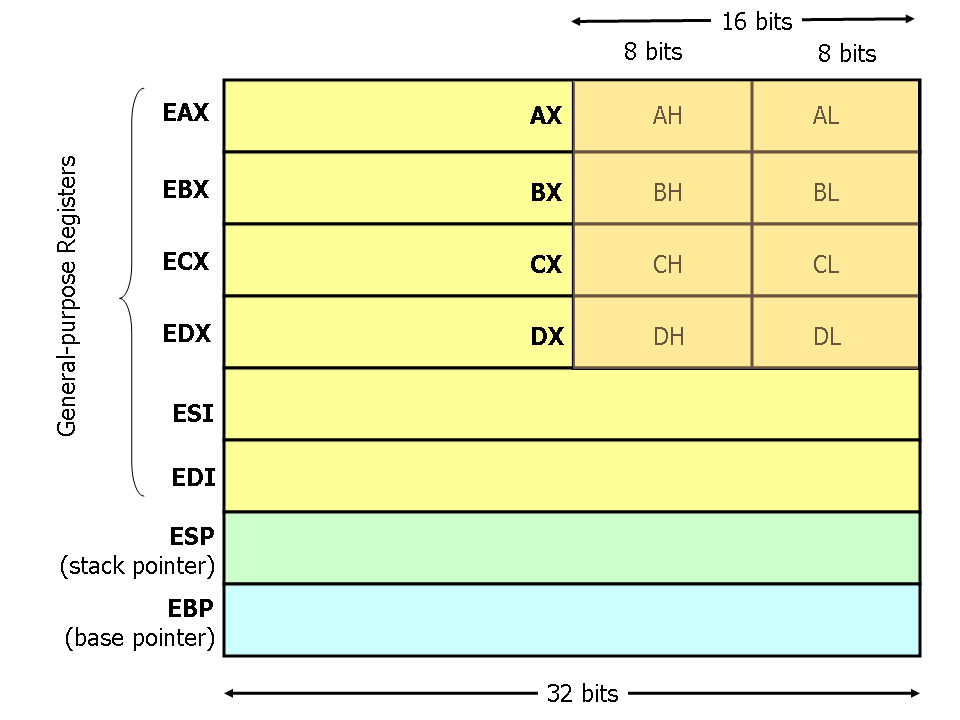
\includegraphics[width=0.7\textwidth]{ImagenesApunte/registrosX86.png}
    \caption{Parte de los registros de x86, tener en cuenta para el TP de JOS}
\end{figure}

\subsubsection*{El Stack}

En la arquitectura x86 los programas utilizan el stack del programa para soporta la llamada a funciones. La maquina utiliza el stack para:
\begin{itemize}
    \item pasar la información de los parámetros.
    \item almacenar la información de retorno.
    \item almacenar los valores de ciertos registros para su posterior utilización.
    \item para almacenamiento local.
\end{itemize}

La porción del stack para realizar esto se llama \textit{stack frame}. La estructura del stack frame esta delimitada por 2 valores, el stack frame pointer, registro \%EBP y el stack pointer, registro \%ESP. El stack pointer puede moverse durante la ejecución de la función, toda la información es accedida en forma relativa con el stack frame pointer.

El conjunto de registros de un procesador es una fuente limitada de recursos que son compartidos por las distintas funciones que se están ejecutando. Cuando se ejecuta una función, hay que asegurarse que la función que llama (caller) a otra función (callee), esta ultima no sobre escriba todos los valores de los registros, ya que algunos de estos van a ser necesitados por la función llamadora. Por lo tanto se define una convención. 

\begin{itemize}
    \item Los registros \%EAX, \%EDX y \%ECX son denominados Caller-save, es decir, cuando Q es llamado por P, el llamador puede sobre-escribir esos registros sin miedo de destruir datos de P.
    \item Los registros \%EBX, \%ESI y \%EDI son denominados Callee-save, esto significa que Q debe guardar los valores de estos registros en la pila antes de sobrescribirlos y restaurarlos antes de retornar
\end{itemize}

\section{El proceso}
\subsection*{La compilación}
Esta compuesta por 4 fases.
\begin{itemize}
    \item La fase de procesamiento: El preprocesador (cpp) modifica el código fuente original del programa escrito en C comenzando con las directivas (\#). El resultado es otro programa C (.i).
    \item La fase de compilación: El compilador (cc) traduce el programa .i a un archivo .s que tiene el programa en assembly.
    \item La fase de ensamblaje: El ensamblador traduce el .s en lenguaje de maquina y los almacena en un formato como programa objeto relocable (.o).
    \item La fase de link edición: Junta las bibliotecas utilizadas.
\end{itemize}

\begin{figure}[!htb]
    \centering
    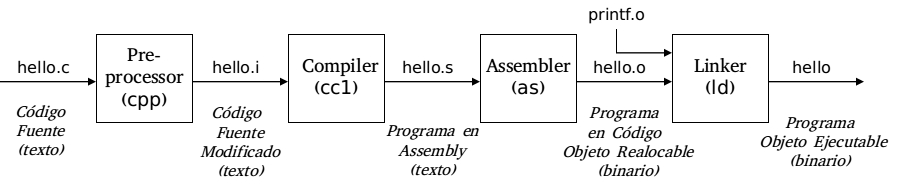
\includegraphics[width=0.9\textwidth]{ImagenesApunte/compilation.jpg}
\end{figure}

\subsection*{El programa en UNIX}
Un programa es un archivo que tiene toda la información de como construir un proceso en memoria. Este contiene:
\begin{itemize}
    \item Formato de identificación binaria: Es la META información que describe el formato ejecutable. Le permite al kernel interpretar la información contenida en el mismo archivo.
    \item Instrucciones de Lenguaje de Maquina: Almacena el código del algoritmo del programa.
    \item Dirección del punto de entrada del programa: Indica la dirección de la primera instrucción que el programa debe ejecutar.
    \item Datos: Son los valores con los que se deben inicializar variables, constantes, y literales.
    \item Símbolos y Tablas de Realocación: Describe la ubicación y los nombres de las funciones y variables del programa. Tiene otra información para debug también.
    \item Bibliotecas compartidas: Describe los nombres de las bibliotecas compartidas que son usadas durante la ejecución. También tiene la ruta del linker dinámico que debe ser usado.
    \item Otra información necesaria para terminar de construir el proceso en memoria.
\end{itemize}

Un programa es algo 'sin vida', un conjunto de instrucciones y datos que esperan en algún lugar del disco para saltar a la acción. El OS es quien lo toma y lo transforma en algo útil, mediante el Kernel.

\textit{a.out es assembly output}

El Kernel realiza lo siguiente.
\begin{enumerate}
    \item Cargar instrucciones y Datos de un programa ejecutable en memoria.
    \item Crear el Stack y el Heap
    \item Transferir el Control al programa
    \item Proteger al SO y al Programa
\end{enumerate}


\subsection*{El proceso}

'Un proceso es la ejecución de un programa de aplicación \textit{con derechos restringidos}; el proceso es \textit{la abstracción} que provee el Kernel del sistema operativo para la ejecución protegida'- [DAH]

El con derechos restringidos nos dice que esta en una maquina con dual mode, y que se ejecuta en el ring 3. La abstracción equivale a la virtualización que se tiene, que provee el kernel.

Un proceso en realidad es mas que un simple programa en ejecución. Un proceso incluye muchas mas cosas.
\begin{itemize}
    \item Los archivos abiertos
    \item Señales pendientes
    \item Datos internos del kernel
    \item El estado completo del procesador
    \item Un espacio en memoria
    \item Uno o mas hilos en ejecución, los cuales tienen su contador de programa, stack, y registros
    \item Datos globales
\end{itemize}

\textit{Leer: No silver Bullet – Essence and Accident in Software Engineering}

\subsection*{La virtualización}

Es crear una abstracción que haga que un dispositivo de hardware sea mucho mas fácil de utilizar.

En los OS modernos se proporciona la virtualización de memoria y del procesador.

\subsubsection*{En memoria}
La virtualización de memoria le hace creer al proceso que este tiene toda la memoria disponible para ser reservada y usada como si este estuviera siendo ejecutado sólo en la computadora. Estos se dividen en texto (instrucciones del programa (.text o .code)), .data (variables globales), el heap, y el stack. Estas secciones se llaman espacio de direcciones del proceso. Están guardadas y el kernel sabe cuales son. Apenas el proceso quiere salir de esa sección de memoria, el kernel le tira una interrupción.

\begin{figure}[!htb]
    \centering
    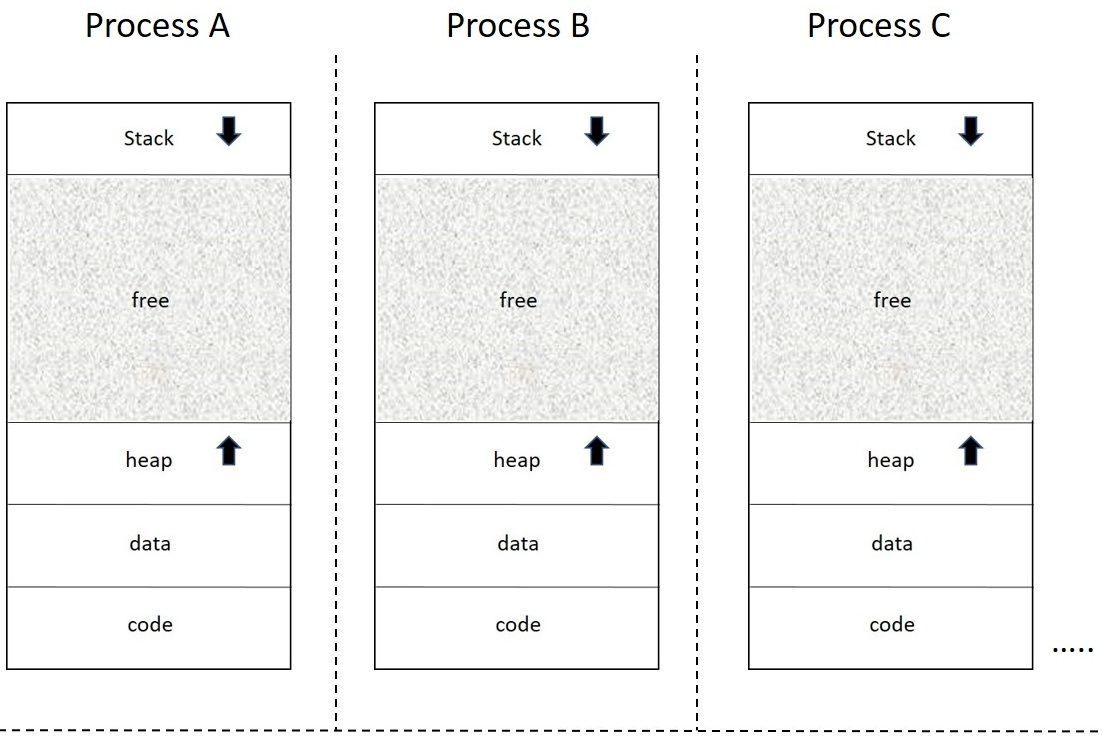
\includegraphics[width=0.7\textwidth]{ImagenesApunte/procesosMemoria.png}
\end{figure}

Para que un proceso se ejecute tiene que estar residente en memoria junto con el sistema operativo. Incluso pueden estar otros procesos simultáneamente. Para lograr esto, el OS tiene que configurar el hardware de forma tal de que cada proceso solo pueda ver y escribir lo suyo. El hardware provee mecanismos de protección para esto.

Uno de los mecanismos es la memoria virtual, esta es una abstracción por al cual la memoria física puede ser compartida por diversos procesos. El componente clave en este caso son las direcciones virtuales, para cada procesos su memoria empieza en el mismo lugar, la dirección 0. Esto hace que cada proceso piense que tiene toda la memoria para el.

El mapeo de una dirección virtual a una física ocurre a través del hardware con una Memory Managment Unit (MMU).

\begin{figure}[!htb]
    \centering
    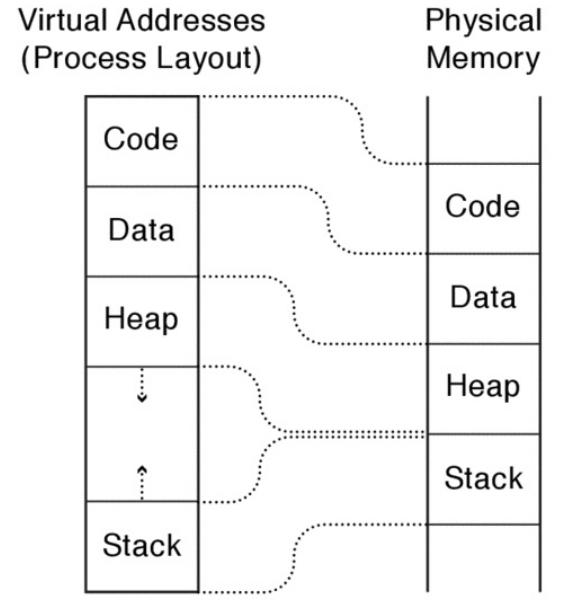
\includegraphics[width=0.7\textwidth]{ImagenesApunte/virtualizacionMemoria.jpg}
\end{figure}

\subsubsection*{En CPU}
La virtualización del procesador es la forma de virtualización más primitiva, consiste en dar la ilusión de la existencia de un único procesador para cualquier programa que requiera de su uso.

\begin{figure}[!htb]
    \centering
    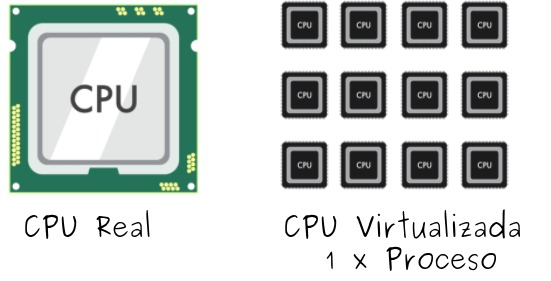
\includegraphics[width=0.55\textwidth]{ImagenesApunte/virtualizacionCpu.jpg}
\end{figure}

Esto permite que cada proceso crea que tiene toda la CPU y que le pertenecen todos los dispositivos. También provee una ilusión en cuanto a que todos los dispositivos tiene el mismo nivel de interfaces y que son mas potentes para su uso.

Otra ventaja de este sistema es que otorga un gran aislamiento ante fallas, ya que los procesos no pueden afectar directamente a otros procesos, y los errores no colapsan toda la maquina.

Esta gran ilusión se crea mediante el kernel.

\begin{figure}[!htb]
    \centering
    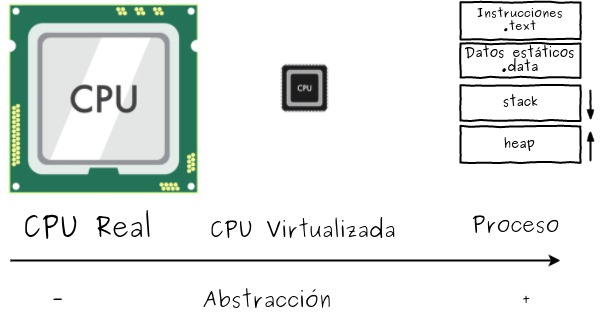
\includegraphics[width=0.7\textwidth]{ImagenesApunte/cpuvirtualizacion2.jpg}
\end{figure}

\subsection*{El proceso por dentro}

La idea general detrás de la abstracción es la de cómo virtualizar una CPU o procesamiento, es decir cómo hacer para que un único procesador actúe como tal para varios programas que requieren ser ejecutados utilizando el mismo hardware.

Cualquier proceso necesita permisos del kernel para poder realizar cualquiera de las siguientes acciones.
\begin{itemize}
    \item Acceder a memoria de otro proceso
    \item Escribir o leer en el disco
    \item Cambiar algún seteo del hardware.
    \item Enviar información a otro proceso.
\end{itemize}

\subsubsection*{API}
\begin{itemize}
    \item Create: fork(), un proceso en UNIX se crea siempre a partir de otro proceso.
    \item Destroy: exit(), kill()
    \item Wait: wait()
    \item Controles varios: exec(), sbrk() (aumenta el address space en malloc())
    \item Status: getpid(), getppid()
\end{itemize}

\subsubsection*{El contexto}
Cada proceso tiene un contexto bien definido que tiene toda la información necesaria para describirse.
\begin{itemize}
    \item User Address Space: text, data, stack, y heap
    \item Control Information: el kernel utiliza dos estructuras principales para mantener la información contenida: la \textit{u area} y \textit{proc}. Cada proceso tiene su propio kernel stack y mapas de traducción de direcciones.
    \item Credentials: son las ids del proceso asociado a el, de grupos y de usuario.
    \item Variables de entorno: strings variables heredadas del padre.
    \item Hardware context: es el contenido de los registros de propósito general, junto con algunos registros especiales del sistema (PC, SP, PWD, registros del manejo de memoria, y de la unida de punto flotante).
\end{itemize}

\begin{minted}{C}
    // the registers xv6 will save and restore
    // to stop and subsequently restart a process
    
    struct context
    {
        int eip;
        int esp;
        int ebx;
        int ecx;
        int edx;
        int esi;
        int edi;
        int ebp;
    };
    
    // the different states a process can be in
    enum proc_state { UNUSED, EMBRYO, SLEEPING, RUNNABLE, RUNNING, ZOMBIE };
    
    // the information xv6 tracks about each process
    // including its register context and state
    struct proc {
        char *mem;                  // Start of process memory
        uint sz;                    // Size of process memory
        char *kstack;               // Bottom of kernel stack
                                    // for this process
        enum proc_state state;      // Process state
        int pid;                    // Process ID
        struct proc *parent;        // Parent process
        void *chan;                 // If non-zero, sleeping on chan
        int killed;                 // If non-zero, have been killed
        struct file *ofile[NOFILE]; // Open files
        struct inode *cwd;          // Current directory
        struct context context;     // Switch here to run process
        struct trapframe *tf;       // Trap frame for the
                                    // current interrupt
    };
\end{minted}

\subsubsection*{U Area y Proc}
Estas dos estructuras dependen de la implementación misma del kernel.

La proc structure es una entrada en la process table. Contiene información a la cual se puede acceder cuando el proceso no se esta ejecutando. Contiene el PID, ubicacion del mapa de direcciones del kernel del u area del proceso, el estado actual, prioridad, información para el manejo de señales. Es conocido también como \textit{task structure} en Linux.

La U area (user area) es parte del espacio del proceso. Esta es vista solo por el proceso cuando esta siendo ejecutado. Contiene Process Control Block (guarda el hardware context cuando el proceso no se ejecuta), un puntero a la proc structure, argumentos para, y retorno o errores hacia la system call actual, manejadores de señales, información de las areas de memoria, tabla de open fd.

\subsubsection*{fork}
Crea un nuevo proceso. Para esto se realizan varias acciones.
\begin{itemize}
    \item Se chequea que hay recursos.
    \item Obtiene una entrada en la  Process Table (PID unico).
    \item Verifica que no se ejecuten demasiados procesos.
    \item Cambia el estado del proceso hijo a 'siendo creado'. Permite que el scheduler no le haga nada, ya que lo esta creando el kernel.
    \item Copia datos de la process table del padre al hijo.
    \item Aumenta contadores (directory inode, file table).
    \item Hace una copia del contexto del padre en memoria.
    \item Crea un contexto a nivel sistema falso para el hijo. (para que el hijo se reconozca y tenga un punto de inicio)
\end{itemize}

Ambos procesos ocurren de forma concurrente, haciendo que no haya determinismo en el orden de ejecución. (Están vivos al mismo tiempo)

Ejemplo del Arpaci.
\begin{minted}{C}
    #include <stdio.h>
    #include <stdlib.h>
    #include <unistd.h>
    
    int main(int argc, char *argv[])
    {
        printf("hello world (pid:%d)\n", (int) getpid());
        int rc = fork();
        if (rc < 0) {// fork failed; exit
            fprintf(stderr, "fork failed\n");
            exit(1);
        } else if (rc == 0) { // child (new process)
            printf("hello, I am child (pid:%d)\n", (int) getpid());
        } else { // parent goes down this path (main)
            printf("hello, I am parent of %d (pid:%d)\n", rc, (int) getpid());
        }
        return 0;
    }
\end{minted}


\subsubsection*{exit}
Esta system call realiza:
\begin{itemize}
    \item Ignora todas la signals
    \item Cierra todos los archivos abiertos
    \item Se liberan los locks sobre los archivos
    \item Libera el directorio actual
    \item Se separan segmentos de memoria compartida
    \item Se actualizan contadores
    \item Libera memoria
    \item Pone el estado del proceso en modo zombie, asignándole como proceso padre a init, casi toda la información del proceso murió, queda algo de meta-data solamente.
    \item Manda señal de muerte al proceso padre 
    \item Context switch
\end{itemize}



\subsection*{Estados}
De forma simple se puede mostrar como sigue, en realidad hay mas estados posibles.
\begin{itemize}
    \item Running
    \item Ready
    \item Blocked
\end{itemize}

El que hace que pase de ready a running es el planificador.

\begin{figure}[!htb]
    \centering
    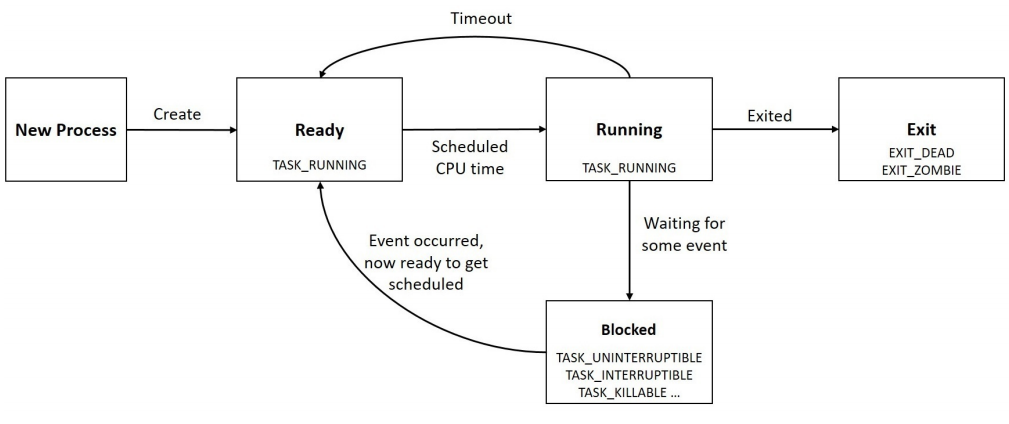
\includegraphics[width=0.8\textwidth]{ImagenesApunte/EstadosLinux.png}
    \caption{Estados en los que puede estar un proceso en Linux}
\end{figure}

\newpage



%lab shell
% hay un esqueleto, relacionado en el parseo de las lineas
% shell, tiene que ser un programa robusto, tolerante a fallos, estan puestos varios de los free, en alguna parte tenemos que llamarlo
% shell, hace un fork, y un exec con el comando
% si le agregamos redireccion, pipes se vuelve mas complejo
% inicia - toma la linea, parsea el comando, lo ejecuta, espera (proceso de shell a comando), y vuelve a empezar desde la linea - despues se cierra, termina en algun punto

% Parte 1
% proceso en segundo plano, modificar el wait, & al final indica de ejecutar un proceso en segundo plano
% challenge opcional, notificar correctamente cuando finaliza el segundo procesos

% Parte 2
% dup(2) duplica un file descriptor
% dup2() se le pasa un old fd (donde se quiere redireccionar el flujo estandar) y un nuevo fd(el fd que se quiere redireccionar). Si estaba siendo usado, lo cierra y lo redirecciona.
% dup2 es atomico, conviene mas que dup y close
% <> van pegados al nobmre del archivo Ej >out.txt <in.txt
% 2>&1 El & para redireccionar a otro fd desde la shell
% pipes, se toma el stdout de uno y se remplaza el stdin del otro - estan sincronizados de forma inherente (uno escribe, el otro lee) el que lee esta esperando
% el proceso que une dos nodos (ijos unidos entre si con un pipe)
% los procesos no se lanzan de a uno con el pipe, se lanzan todos y estan sincronizados con el pipe
% el promt no tiene que volver enseguida, tiene que terminar todo el comando entero para que termine exec command, y la shell pueda devolver el promt al usuario.

% sh.c es el punto de entrada -> runcmd.c
% parse line para las tuberias multiples
% exec en execcmd.c

% EXEC es el caso simple, ejecuta un comando con 0 o muchos argumentos

%%%%%%% PARTE 3 : VARIABLES DE ENTORNO
% $PATH
% $LS_COLORS <----------- PROBAR
% ocurre antes de la ejecucion, echo $PATH busca la variable, y se la pasa como argumento al comando echo
% Si comienza con $, buscamos el valor de la variable y la sobreescribimos - getenv(3) (sin el $) 
% echo $NO_EXISTE - imitar el comportamiento
%
% hacer un realloc() al agregar el value devuelto
% export NO_EXISTE=hola
% echo $NO_EXISTE
% hola
% al realizar el export se crea una variable temporal disponible para todos los procesos que se ejecuten en esa terminal
% HOLA=hola /env/var/... | grep al
% agrega la variable temporal solamente durante ese momento, se incorporan nuevas variables, queremos que esten solo disponibles para el proceso nuevo que queremos correr -setenv(3) , unsetenv(3)
% entre el fork y el exec realizar el setenv(), hace que la duracion este solamente relacionada con la vida del proceso ese
% execle() y execvpe() permiten settear el environment de lo que se esta por ejecutar, sin el 'e' los procesos heredan las variables de entorno de otro proceso de la shell
% variables 'magicas' son casos de variables que son especificas de la shell, no de entorno del proceso
% $_ el valor del ultimo argumento del ultimo comando
% $$ indica el pid del proceso que se esta corriendo actualmente
% $? tiene el status code del ultimo proceso en ser ejecutado - DEL ULTIMO (en los | prestar atencion)
% 
% PARTE 4: BUILTIN
% se ejecutan en el mismo proceso de la shell
% man true - man false 
% man strace - strace ps - muestra toda syscall que uso el proceso - muy bueno para hacer debug!
% kill sirve para mandar cualquier tipo de señal a algun proceso tambien! (ademas de terminarlos) - al matar a un proceso, se saca el proceso de las estructuras internas del kernel, ya no utiliza recursos, libera todo! el tema es que no deje cosas corruptas, que quede un socket esperando informacion, que no deje efectos secundarios.
% jobs para ver los procesos en segundo plano
% yes mensaje, imprime un mensaje por pantalla infinitas veces
% /proc no es un directorio normal, en el cual no podemos crear archivos, /proc/version tiene tamaño 0 - O_O - /proc/kcore tamaño de terabytes, es el espacio virtual
% no es un directorio que este soportado en disco, se conoce como un pseudo-filesystem de tipo proc, el kernel intercepta cualquier syscall sobre ese directorio, y nos responde lo que quiera con parte de sus estructuras internas. VENTANAS A LAS ESTRUCTURAS INTERNAS DEL KERNEL - /proc de solo lectura, hay otros de solo escritura que cambian configuracion del kernel
% mount y unmount para ver el proc en cualquier directorio - el kernel te hace ver cosas que no estan


%En linux todo es un proceso, y los tasks se refieren a ellos tambien. Cada proceso con su informacion, esto esta guardado dentro de un struct task (que es enorme - +2kb de memoria).


\section*{Quinta y sexta clase}
\section{La memoria}
El  tema principal sobre la administración de la memoria se encuentra en como representarla.

La memoria física se imagina como un arreglo de direcciones de memoria.

Esto resulta manejable mientras la cantidad de memoria este en un rango adecuado, dado por la arquitectura.

\subsection*{Address Space}
Crear un mecanismo que permita que la memoria física de una computadora sea utilizada de forma fácil y eficiente llevo paulatinamente a concebir el concepto de espacio de direcciones, la abstracción para la memoria.

El Address Space de un proceso contiene todo el estado de la memoria de un programa en ejecución.

\begin{figure}[!htb]
    \centering
    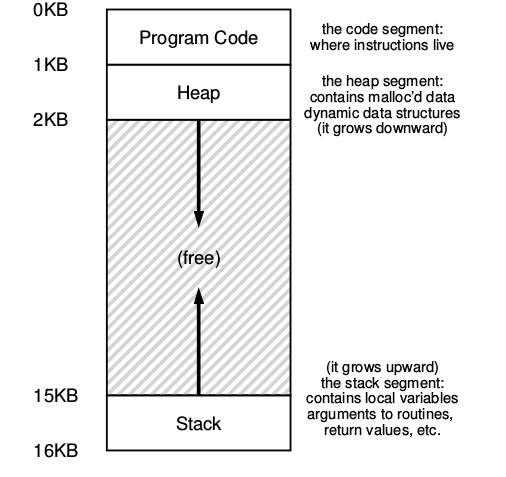
\includegraphics[width=0.6\textwidth]{ImagenesApunte/address_space.jpg}
\end{figure}

Cuando se esta describiendo así el espacio de direcciones, se esta describiendo la abstracción que provee el sistema operativo, ya que el programa piensa que esta cargado a partir de la dirección 0 y que tiene toda la memoria para el.

Cuando por ejemplo un proceso trata de cargar el contenido de la dirección 0 (la dirección virtual 0), de alguna forma el sistema operativo con ayuda de algún tipo de mecanismo de hardware que tendrá que asegurarse que no se cargue la dirección física 0 real más bien que se cargue la dirección física en la cual el espacio de direcciones de ese proceso se encuentra alojado.

Esta implementación de la memoria virtual esta hecha de forma tal de que sea invisible al programa que se ejecuta, pero detrás de escena, el OS y el hardware llevan a cabo la ilusión.

Otras cuestiones importantes de la implementación son el tiempo (que los programas no sean mas lentos) y el espacio (no usar demasiada memoria para las estructuras de la memoria virtual), la memoria virtual debe ser eficiente.

La ultima cuestión que debe de tener es la de la protección. El OS debe de asegurarse de proteger a los procesos entre si, y de protegerse a si mismo. Esto habilita el aislamiento entre procesos.

\subsection*{La API}
En un programa en ejecución existen 2 tipos distintos de memoria, el heap y el stack.
\begin{itemize}
\item La del stack es reservada y liberada implícitamente por el compilador. Su declaración es a través de la declaración de variables.
\item La del heap se obtiene y libera explícitamente por el programador. \textit{Ej. malloc() y free()} Estas funciones internamente hacen llamadas a las syscalls \textit{brk() y sbrk()}
\end{itemize}

\subsection*{Traducción}
Se hace a través de una técnica llamada Hardware-Based Address Translation, o directamente Address Translation. 

Esta técnica transforma la dirección virtual en una física. El hardware provee un mecanismo eficiente de bajo nivel, y el sistema operativo setea al hardware de la forma correcta, gerencia la memoria manteniendo información de los lugares libres y en uso, y mantiene el control sobre la memoria usada.

\begin{figure}[!htb]
    \centering
    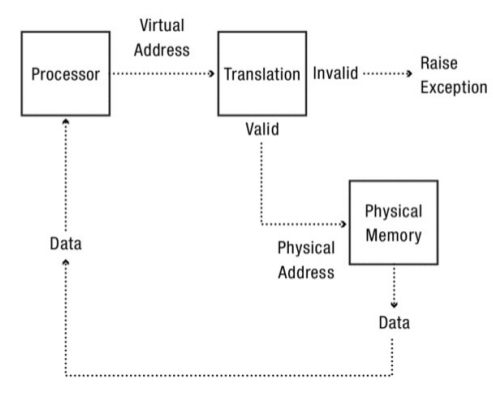
\includegraphics[width=0.6\textwidth]{ImagenesApunte/address_translation_function.jpg}
\end{figure}

Cuestiones que provee la traducción de las direcciones
\begin{itemize}
\item Aislamiento de procesos
\item Comunicación entre procesos, si los procesos deben de coordinar-se entre si, una forma eficiente de hacerlo es que tengan una región compartida de memoria. 
\item Segmentos de código compartidos para instancias de un mismo programa, haciendo mas eficiente el uso de la cache.
\item Inicialización de programas, se puede empezar un programa antes de que se haya cargado a memoria todo el código.
\item Uso eficiente de la memoria de forma dinámica
\item Administración de la cache, ubica los programas en memoria física de forma eficiente para que mejore la eficiencia del cache. Se hace con un sistema llamado \textit{Page coloring}
\item Debugging de programas, puede evitar que programas con bugs sobre escriban secciones de su propio código, atrapando el error de forma temprana.
\item Uso eficiente de I/O
\item Archivos mapeados a memoria
\item Memoria virtual
\item Puntos de control y reinicio, el estado de un programa puede ser guardado de forma periódica en caso de que se rompa el programa o sistema. Esto permite que se pueda reiniciar de ese punto guardado.
\item Estructuras de datos persistentes
\item Migración de procesos
\item Control del flujo de la información, actúa como una capa de seguridad extra, para evitar que se envié información a donde no tiene que ir.
\item Distribución de la memoria compartida
\end{itemize}


\subsection*{Dynamic Realocation o Memoria segmentada}
\subsubsection*{Base and Bound}
Se necesitan dos registros, el \textit{base} y el \textit{limite o segmento}. Estos registros permiten que el address space pueda ser ubicado en cualquier lugar de la memoria física.

\begin{math}
PhysicalAddress = VirtualAddress + base
\end{math}

El registro bound (limite o segmento), es verificado antes de realizar alguna operación en memoria.

\begin{figure}[!htb]
    \centering
    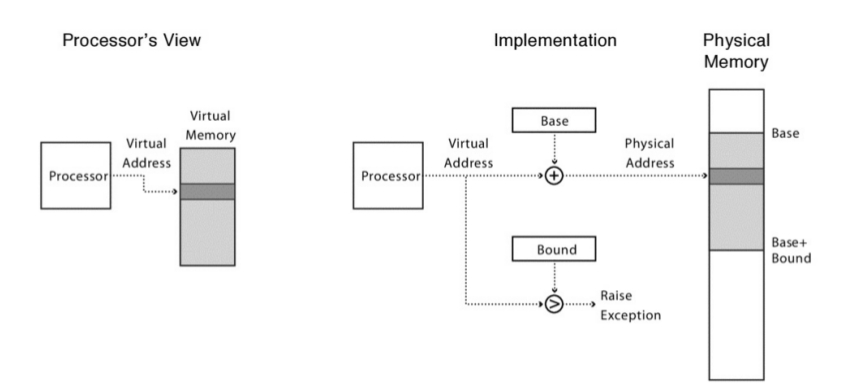
\includegraphics[width=0.8\textwidth]{ImagenesApunte/base_bound.jpg}
\end{figure}

Esto forma parte edd la MMU (Memory Managment Unit)

\subsubsection*{Tabla de segmentos}
El problema de Base and Bound es que se tiene un solo registro base y un solo segmento. Se mejora teniendo un arreglo de pares base-segmento por cada proceso,  donde cada entrada controla una parte del virtual address space.

\begin{figure}[!htb]
    \centering
    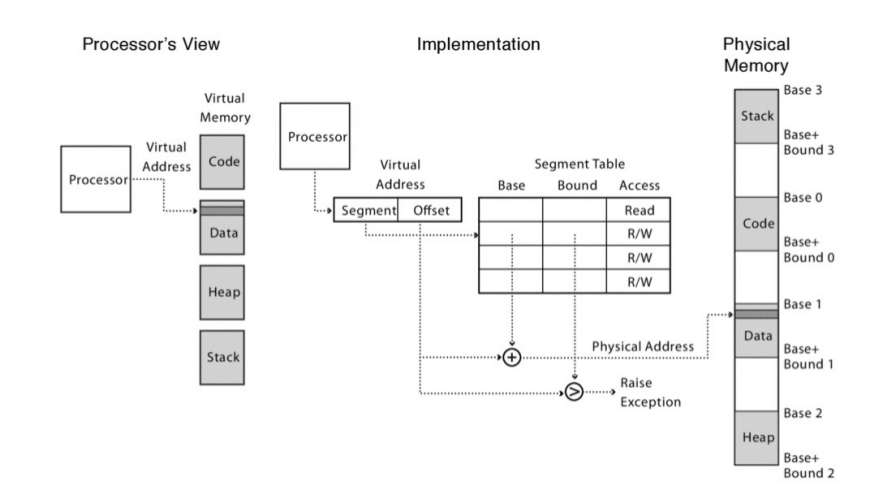
\includegraphics[width=0.8\textwidth]{ImagenesApunte/segment_table.jpg}
\end{figure}

Las direcciones virtuales tienen un numero de segmento (index) y un offset.

Se tienen bits de protección también, lectura, escritura, ejecución.

Segmentación de grano fino vs segmentación de grano grueso. La primera consiste en tener muchos segmentos pequeños y la segunda consiste en tener pocos segmentos grandes.

El problema de la segmentación es la fragmentación, precisamente la fragmentación externa.

\subsubsection*{Paginada}
En este caso la memoria se reserva en pedazos de tamaño fijo llamados page frames. La traducción se realiza de forma similar al segmentada. (4KB generalmente)

Hay una tabla de paginas por cada proceso con punteros a las page frames. Como tienen un tamaño fijo, y son potencia de 2,las entradas en la page table sólo tienen que proveer los bits superiores de la dirección de la page frame. De esta forma van a ser más compactos. No es necesario tener un límite; la página entera se reserva como una unidad.

\begin{figure}[!htb]
    \centering
    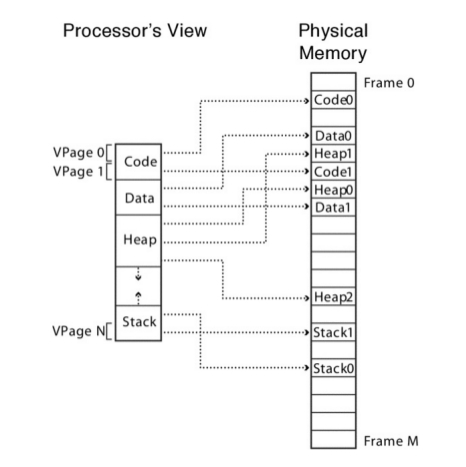
\includegraphics[width=0.5\textwidth]{ImagenesApunte/logical_view_page_address.jpg}
    \caption{El modelo en la memoria.}
\end{figure}

\begin{figure}[!htb]
    \centering
    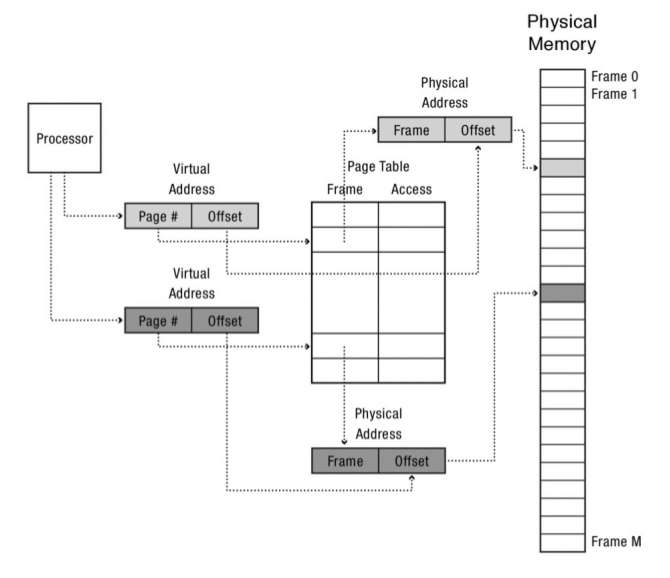
\includegraphics[width=0.7\textwidth]{ImagenesApunte/address_translation_with_page_table.jpg}
    \caption{El proceso de traducción con memoria paginada.}
\end{figure}

\newpage
\subsubsection*{Multinivel}
Es un mecanismo mas eficiente de paginación, basado en un árbol o hash table. Proporcionan
\begin{itemize}
    \item Protección de memoria de grano fino
    \item Memoria Compartida
    \item Ubicación de memoria flexible
    \item Reserva eficiente de memoria
    \item Un sistema de búsqueda de espacio de direcciones eficiente
\end{itemize}

\subsubsection*{Segmentación paginada (paged segmentation)}
Este sistema usa dos niveles de un árbol. Con paged segmentation, la memoria esta segmentada, pero en vez de que cada entrada en la pagina de segmentos apunte directamente a una región continua de la memoria física, cada entrada en la tabla de segmentos apunta a una tabla de paginas, que a su vez apunta a la memoria correspondiente a ese segmento. La tabla de segmentos tiene una entrada llamada limite o tamaño que describe la longitud de la pagina de tablas, osea la longitud de los segmentos en las paginas

Existen también casos con mas niveles, y sistemas de hash.

\begin{figure}[!htb]
    \centering
    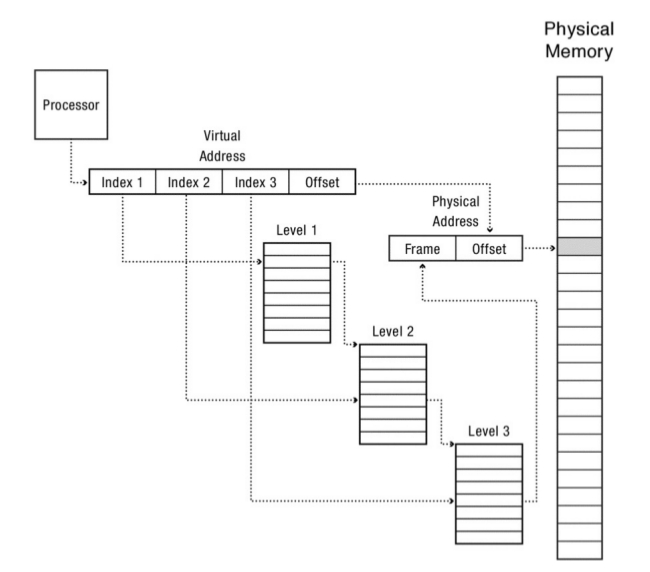
\includegraphics[width=0.7\textwidth]{ImagenesApunte/address_translation_with_three_level.jpg}
    \caption{El proceso de traducción con tres niveles.}
\end{figure}

\newpage

\subsection*{Mejora del rendimiento: TLB}
Como se vio que había mejoras de localidad y temporalidad, se utiliza un cache llamado Translation-Lookaside Buffer el cual es parte de la MMU. Este sistema guarda los pares de direcciones virtuales a físicos utilizadas. Por cada referencia a memoria, el hardware se fija primero la TLB. Si esta guardada la referencia (TLB hit), va a memoria sin tener que realizar la traducción, resultando un proceso mas rápido. (ya que la traducción es ir a buscar a memoria la tabla, TLB miss)

Una cuestión a tener en cuenta es la consistencia con los datos originales cuando las entradas son modificadas.

En general tienen 32-64 entradas.

\begin{itemize}
\item El context switch: Las direcciones virtuales de un viejo proceso ya no son más válidas, y no deben ser válidas para el nuevo proceso. De otra forma, el nuevo proceso sería capaz de leer las direcciones del viejo proceso. Frente a un context switch, se necesita descartar el contenido de TLB en cada context switch. Este approach se denomina flush de TLB. Debido a que este proceso acarrearía una penalidad, los procesadores taguean la TLB de forma tal que la misma contenga el id del proceso que produce cada transacción.
\item Reducción de Permiso: Qué sucede cuando el sistema operativo modifica una entrada en una page table? Normalmente no se provee consistencia por hardware para la TLB; mantener la TLB consistente con la page table es responsabilidad del sistema operativo.
\item TLB shutdown: En un sistema multiprocesador cada uno puede tener cacheada una copia de una transacción en su TLB. Por ende, para seguridad y correctitud, cada vez que una entrada en la page table es modificada, la correspondiente entrada en todas las TLB de los procesadores tiene que ser descartada antes que los cambios tomen efecto. Típicamente sólo el procesador actual puede invalidar su propia TLB, por ello, para eliminar una entrada en todos los procesadores del sistema, se requiere que el sistema operativo mande una interrupción a cada procesador y pida que esa entrada de la TLB sea eliminada. Esta es una operación muy costosa y por ende tiene su propio nombre y se denomina TLB shutdown.
\end{itemize}

\subsubsection*{Funcionamiento}

Extraer VPN (Virtual Page Number) de la VA, y chequear si la TLB tiene la traducción para esa VPN. 

\begin{itemize}
\item Si la tiene es TLB HIT.
    \begin{enumerate}
        \item Se extrae la PFN (Page Frame Number) de la entrada de la TLB.
        \item Se concatena el offset de la VA y se tiene la PA, con lo que se puede acceder a memoria.
    \end{enumerate}

				
\item Si fue TLB MISS, haces un page table lookup.
    \begin{enumerate}
        \item El hardware accede a la page table para encontrar la traducción.
        \item Si la referencia a la memoria virtual es valida y accesible, se actualiza la TLB con la traducción nueva.
        \item El hardware vuelve a buscar la instrucción en la TLB, y de ahí ir a la memoria.
    \end{enumerate}
\end{itemize}

\begin{figure}[!htb]
    \centering
    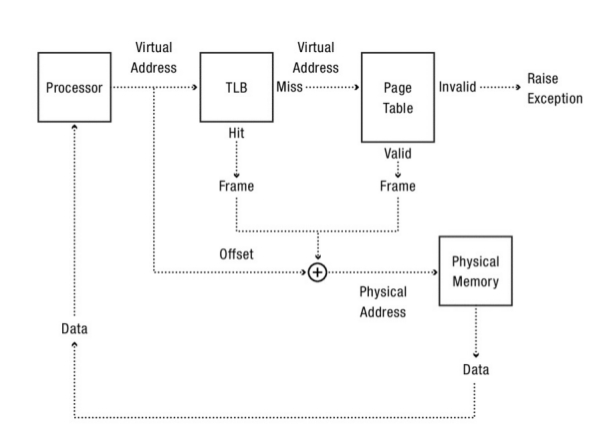
\includegraphics[width=0.7\textwidth]{ImagenesApunte/tlb.jpg}
\end{figure}

\newpage

\section*{Séptima y octava clase}

Nota: Se ve después de memoria por que el TP1 consiste en la implementación de parte del sistema de memoria de JOS.

\section{Scheduling o Planificación de Procesos}

Cuando se tienen muchos programas, tiene que haber alguna forma de poder elegir cual se ejecuta primero o cuanto tiempo de CPU tienen. Este periodo se llama \textbf{time slice} o \textbf{time quantum}. El planificador tiene que tender a O(1), debe de ser lo mas eficiente posible. En el caso de Linux \emph{tiende} a O(1).

\subsection*{Time Sharing}

Surge de la idea de que los programadores tienen la computadora toda para el. Este sistema da la ilusión de que la computadora es toda tuya, pero no es así. Se comparte el tiempo de procesamiento.

\subsubsection*{Multiprogramación}
Permite que si alguien esta haciendo E/S alguien mas haga computo.
\subsubsection*{Uso del CPU}
Si un determinado programa que se estaba ejecutando debía realizar operaciones de entrada y salida de datos, debía interactuar con un dispositivo de entrada y salida. Esta interacción en términos de tiempos de ejecución de instrucciones del procesador podía parecer infinito. Además, con el agravante de que el tiempo de E/S solía ser en promedio de entre el 80\% y 90\% del tiempo total del programa, la CPU permanecía inactiva un gran período de tiempo.

\textit{Ej. Si se asume que el 20\% del tiempo de ejecución de un programa es solo cómputo y el 80\% son operaciones de entrada y salida, con tener 5 procesos en memoria se estaría utilizando el 100\% de la CPU.}

El cálculo es más realista si se supone que un proceso gasta una fracción p, bloqueado en E/S. Por lo tanto, la probabilidad de que $n$ procesos estén en E/S es $p^n$. Entonces, el uso del procesador queda definido como $1-p^n$.

\subsubsection*{Multiple Fixed Partitions}
Dividís en particiones la memoria, y los procesos se asignaban a esas particiones. En una se ejecutan los procesos grandes (partición grande) y en otras particiones chicas los procesos mas chicos. El problema esta en cuanto se acaba uno de los tipos, si tengo muchos procesos chicos tengo mucho espacio de memoria (de partición grande) desperdiciado.

\textit{Leer 'An Experimental Time-Sharing System' de Corbato.}

\subsubsection*{Multiple variable Partitions}
Cada tarea entra en memoria y ocupa un espacio. En este caso se puede realocar la memoria donde hay un espacio para aprovecharla mejor (reubica para reducir la fragmentación interna de la memoria). Esto elimina la fragmentación interna y externa.


\subsection*{Time Sharing}

Cuando un Sistema Operativo se dice que realiza multi-programación de varios procesos debe existir una entidad que se encargue de coordinar la forma en que estos se ejecutan, el momento en que estos se ejecutan y el momento en el cual paran de ejecutarse. En un sistema operativo esta tarea es realizada por el Planificador o Scheduler que forma parte del Kernel del Sistema Operativo.

\subsection*{Workload}
Es la carga de trabajo de un proceso corriendo en el sistema. Normalmente a los procesos se les dice \emph{jobs}.


\subsection*{Metricas}
Para poder hacer algún tipo de análisis se necesitan métricas para poder comparar diferentes políticas de planificación.

\subsubsection*{Turnaround}
Es el tiempo en que se completa un \emph{job} menos el tiempo en que llega. Normalmente la unidad de tiempo serian nano segundos, para lo que vamos a necesitar la usamos sin unidad.

\begin{center}
\begin{math}
T_{turnaround} = T_{completion} - T_{arrival}
\end{math}
\end{center}

Mide performance, cuan rápido se va a ejecutar un proceso. Si Todos los procesos llegan al mismo tiempo, $T_{arrival} = 0$

\subsubsection*{Tiempo de respuesta}
Nace con el Time Sharing, mide cuan rápido el usuario va a sentir que su proceso se esta ejecutando.

\begin{center}
\begin{math}
T_{response} = T_{firstrun} - T_{arrival}
\end{math}
\end{center}

Surge debido a que los usuarios pretenden interacción con rapidez.


\subsection*{Políticas}
Mientras mas inteligentes son, tienden a tardar mas. Hay que analizar el tradeoff entre la decisión y la la ejecución planificada.

\subsubsection*{First In, First Out - FIFO}
El primero en llegar se ejecuta primero, es un cola. Los problemas que tiene este método es si llega primero un proceso que ocupa una mayor cantidad de tiempo en comparación a los otros. El $T_{around}$ empeora considerablemente. Esto se conoce como \textit{convoy effect}. Esta es una planificación \emph{non-preemptive}, el kernel no puede desalojar un proceso (tiene todo el control del CPU).

\begin{figure}[!htb]
    \centering
    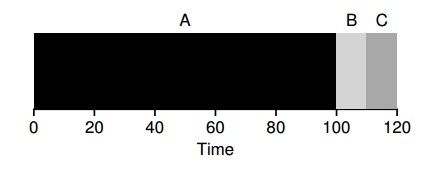
\includegraphics[width=0.6\textwidth]{ImagenesApunte/fifo_convoy.jpg}
\end{figure}

\subsubsection*{Shortest Job First - SJF}
Busca resolver el problema de FIFO. Ejecuta primero el trabajo mas corto. El problema esta en que no se conoce de antemano cuanto va a durar un proceso y que todavía puede llegar un proceso largo sin que haya uno mas corto para ejecutar. También se le sumaria el tiempo que tarda en decidir cual proceso ejecutar. \emph{non-preemptive}


\subsubsection*{Shortest Time-to-Completion - STCF}
En este caso el planificador se adelanta y si hay un proceso que puede terminar antes, ejecuta ese primero, posponiendo la ejecución del que se estaba ejecutando. Esto lo realiza con un context switch. Es \emph{pre-empitve}.

\begin{figure}[!htb]
    \centering
    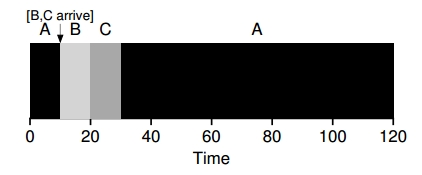
\includegraphics[width=0.6\textwidth]{ImagenesApunte/fifo_stcf.jpg}
\end{figure}

\subsubsection*{Round Robin - RR}
El algoritmo consiste en ejecutar un proceso por un periodo de tiempo determinado (slice), y transcurrido pasar a otro proceso en la cola de ejecución. Trata a todos los procesos igual.

Es importante en este caso elegir un buen time slice. El time slice tiene que amortizar el cambio de contexto sin hacer que esto resulte en que el sistema no responda más.

\textit{Ej. Si el tiempo de cambio de contexto está seteado en 1 ms y el time slice está seteado en 10 ms, el 10\% del tiempo se estará utilizando para cambio de contexto. Sin embargo, si el time slice se setea en 100 ms, solo el 1\% del tiempo será dedicado al cambio de contexto.}

Con este método de planificación, la métrica de $response$ mejora, pero la de $turnaround$ empeora, ya que se atrasa el retorno de todos los programas.

\begin{figure}[!htb]
    \centering
    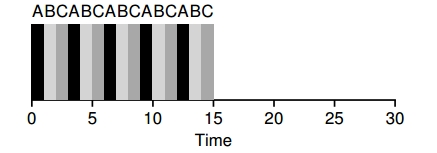
\includegraphics[width=0.6\textwidth]{ImagenesApunte/round_robin.jpg}
\end{figure}

\subsubsection*{Multi-Level Feedback Queue - MLFQ}
Este planificador intenta atacar principalmente 2 problemas.
\begin{itemize}
    \item Intenta optimizar el turnaround time mediante la ejecución de la tarea mas corta primero. (No sabemos cual es)
    \item Intenta hacer que el sistema tenga un tiempo de respuesta interactivo para los usuarios. (Minimizar el response time)
\end{itemize}

Para lograr esto, tiene un conjunto de distintas colas, cada una con un nivel de prioridad distinto.

En un determinado tiempo, una tarea que esta lista para ser ejecutada esta en una única cola. MLFQ usa las prioridades para decidir cual tarea debería correr en un determinado tiempo $t0$. Se puede elegir la tarea con mayor prioridad o la que esta en la cola mas alta.

La clave en este planificador esta en que no otorga prioridades fijas. Estas son variables con el tiempo.

Lo que queremos es que:
\begin{enumerate}
    \item Si una tarea no utiliza el CPU (espera I/O), MLFQ le mantenga una prioridad alta, ya que vendría a ser un proceso interactivo. \emph{Ej. Una tarea espera entrada del teclado.}
    \item Si una tarea usa mucho el CPU, MLFQ le reduzca su prioridad. (No suelta el CPU) \textit{Ej. Cualquier programa que haga mucho calculo.}
\end{enumerate}

\begin{figure}[!htb]
    \centering
    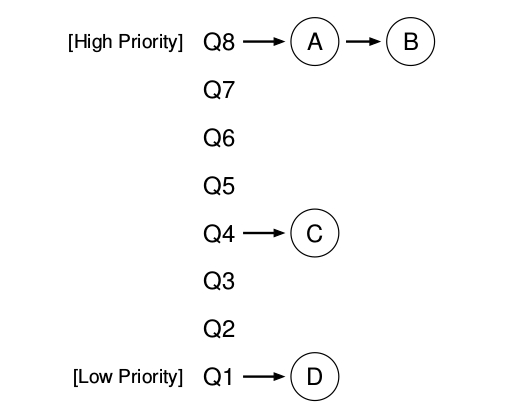
\includegraphics[width=0.6\textwidth]{ImagenesApunte/mlfq.jpg}
\end{figure}

\subsubsection*{Posibles problemas}
Hay que tener algunas consideraciones en la elección de prioridades.
\begin{itemize}
    \item Starvation: Si hay demasiadas tareas interactivas, se van a combinar consumiendo todo el tiempo de la CPU. Esto evitaría que algún proceso que usa mucho la CPU se llegue siquiera a ejecutar.
    \item Un programador podría escribir su programa para que se ejecute mas de lo que debería. \textit{Ej. Se escribe a un archivo que no contiene nada justo antes de que se acabe el time slice.}
    \item Los programas son dinámicos, puede pasar que un programa use mucho el CPU al comienzo y después pase a usar mas I/O, volviéndose mas interactivo.
\end{itemize}

\subsubsection*{Reglas}

Las reglas que tiene MLFQ, siendo A y B dos procesos.
\begin{enumerate}
    \item Si la prioridad de A es mayor que la de B. Se ejecuta A, B no se ejecuta.
    \item Si la prioridad de A es igual a la de B, A y B se ejecutan en Round Robin.
    \item Si entra un proceso nuevo, se le asigna la prioridad mas alta.
    \item Una vez que una tarea usa su asignación de tiempo en un nivel dado, su prioridad se reduce independientemente de si renuncio al CPU. Esto evita que los programadores tomen ventaja del planificador.
    \item Después de cierto periodo S, se mueven todas las tareas a la cola mas alta, se les da un boost de prioridad. Esto arregla el problema de Starvation y de los cambios de formas de ejecución de los programas.
\end{enumerate}

La constante S es una VOO-DOO CONSTANT, requiere de magia negra para ser determinada correctamente. Si S es muy alta, los procesos que requieren mucha ejecución caen en Starvation, si es baja, las tareas interactivas no van a poder compartir correctamente el CPU. La obtención de S es estadístico mediante diferentes pruebas de ejecución.

\begin{figure}[!htb]
    \centering
    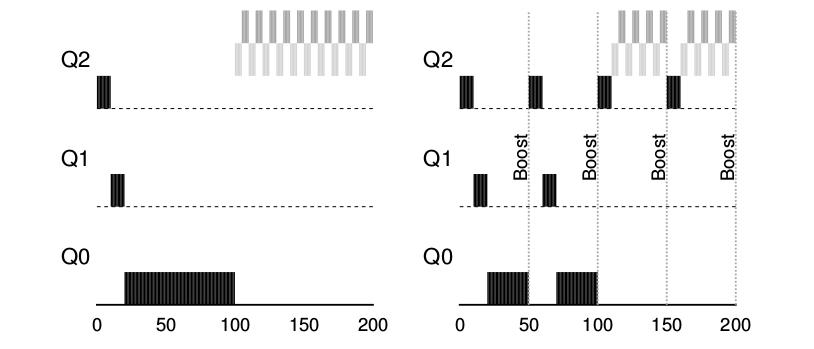
\includegraphics[width=0.7\textwidth]{ImagenesApunte/mlfq_boost.jpg}
\end{figure}

Estas reglas permiten que MLFQ aprenda continuamente sobre los procesos para poder predecir su comportamiento. Hoy en día ya no se utiliza, son mas complejos los planificadores ahora. Se implemento en MULTICS.


\subsubsection*{Proportional Sharing}
Este tipo de planificador cambia la forma en que encara el problema. En vez de optimizar turnaround o response time, intentara que cada tarea obtenga un porcentaje de uso del tiempo de CPU.

El concepto se conoce también como planificación por lotería. Cada cierto tiempo, se hace un sorteo para determinar quien se ejecuta a continuación. Los que deban de ejecutarse mas frecuentemente tienen que tener mas posibilidades de ganar la lotería.

El concepto que subyace en el algoritmo de planificación por lotería es muy básico: los boletos, son utilizados para representar cuanto se comparte de un determinado recurso para un determinado proceso. El porcentaje de los boletos que un proceso tiene es el porcentaje de cuanto va a compartir el recurso en cuestión.

\textit{Ej. Suponiendo que existen dos procesos A y B y que un boleto ganador esta entre 0 y 99 podría suponerse que el proceso A tiene el 75\% de posibilidades de recibir el recurso y el proceso B tiene el 25\% restante. En términos de boletos de la lotería el proceso A tendría los boletos del 0 al 74 y el proceso B tendría los boletos del 75 al 99. UN boleto ganador determina si A o B son ejecutados, entonces el planificador. Entonces por ejemplo de boletos ganadores de la lotería podrían ser: 63 85 70 39 76 17 29 41 36 39 10 99 68 83 63 62 43 0 49 49. Entonces el resultado de la planificación es:
A B A A B A A A A A B A B A A A A A A}

Utilizar la aleatoriedad lleva a una correcta visión desde el punto de vista probabilístico pero no garantiza que esa proporción deseada se lleve a cabo. De hecho en el ejemplo anterior no sucede que se ejecute 25 75. No se garantiza que salgan esos valores.

Existen distintos mecanismos para manipular los boletos.
\begin{itemize}
    \item Ticket Currency: Existen como en la realidad distintos tipos de moneda y las tareas pueden tener los tickets comprados con distintos valores de moneda; el sistema automáticamente los transforma en un tipo global de moneda.
    \item Transferencia de boletos: Este mecanismo permite que un proceso temporalmente transfiera sus boletos a otro proceso. Este mecanismo es útil cuando se esta utilizando la arquitectura cliente/servidor.
    \item Inflación: Con la inflación un proceso puede aumentar o disminuir la cantidad de boletos que posee esto lo puede hacer de forma temporal. Este proceso obviamente no puede realizarse en un sistema en el cual las tareas compiten entre ellas, ya que una tarea muy avara podría captar todos los boletos. Sin embargo, este método puede ser utilizado en un ambiente en el cual los procesos confían entre ellos.
\end{itemize}

Lo interesante de este método es la facilidad con la que se puede implementar. Necesita lo siguiente:
\begin{itemize}
    \item Un buen generador de números aleatorios que determine cual es el numero de la lotería ganador
    \item Una estructura de datos para mantener la información de los procesos del sistema.
    \item Un numero total de tickets.
\end{itemize}

\begin{minted}{C}
    // counter: used to track if we’ve found the winner yet
    int counter = 0;
    
    // winner: use some call to a random number generator to get a value,
    // between 0 and the total # of tickets
    int winner = getrandom(0, totaltickets);
    
    // current: use this to walk through the list of jobs
    node_t *current = head;
    
    // loop until the sum of ticket values is > the winner
    while (current) {
        counter = counter + current->tickets;
        if (counter > winner)
            break; // found the winner
        current = current->next;
    }
    // ’current’ is the winner: schedule it...
\end{minted}

\subsection*{Planificación multiprocesador}
Hoy en día con procesadores multicore hay que planificar de alguna forma también. (Las aplicaciones normalmente nacen secuencialmente y después se las hace multithreading para aprovechar las ventajas que da el multicore). Los planificadores no suelen mejorar el rendimiento de las aplicaciones haciéndolas multithreading, eso queda para el programador. (No tiene la inteligencia de pasar de secuencial a paralelo un programa)

\subsubsection*{Arquitectura multiprocesador}
La diferencia principal se centra alrededor del hardware llamado cache y de que forma los datos que tiene son compartidos a través de los multiprocesadores.

La memoria principal, por el contrario mantienen todos los datos del sistema pero el acceso a los mismos es lento. A través de mantener los datos que son frecuentemente utilizados en la cache, el sistema puede hacer que una memoria larga y lenta parezca una memoria rápida.

Las caches aprovechan la localidad temporal y la espacial.

La localidad temporal se aprovecha cuando cierta cantidad de datos son accedidos, es muy probable que sean accedidos otra vez en un futuro cercano. \textit{Ej. variables o instrucciones que se ejecutan una y otra vez en un ciclo.}

En la localidad espacial cuando un programa que accede a una dirección X es muy probable que necesite volver a acceder cerca de X. Acá podría pensarse en un programa sobre un arreglo. Teniendo en cuenta que este tipo de localidad existe en la mayoría de los programas los sistemas de hardware pueden hacer buen uso de las cache.

\begin{minted}{C}
    for(i = 0; i < 20; i++)
        for(j = 0; j < 10; j++)
            a[i] = a[i]*j;
\end{minted}

En el caso de los multiprocesadores esto se complica, ya que al traer un dato de memoria y guardarlo en su cache, este puede sufrir modificaciones con el tiempo. Supongamos que este programa se cambia a otro procesador por el planificador con un cache diferente, ¿Que sucede con el dato? Puede ocurrir que el programa vaya leer devuelta a memoria el valor viejo si no se tiene cuidado.

Este problema se llama \emph{coherencia del cache}. La solución básica que da el hardware es monitoreando los accesos a memoria, asegurándose que la vista de una memoria única compartida sea preservada. Esto lo puede hacer con una técnica llamada \emph{Bus Snooping}, en donde cada cache pone atención a las actualizaciones de memoria mediante la observación del bus que los conecta. Cuando ocurre algún cambio la CPU anula su propio cache, provocando que se actualice.

\subsubsection*{Afinidad de Cache}
Lo que si sucede en los planificadores, es que cuando el proceso corre sobre una CPU en particular, se va construyendo una parte del estado en la cache de esa CPU. Lo que se intenta hacer es que se mantenga esta afinidad para no tener que reconstruirlo.

Si se ejecutase el proceso en un procesador diferente siempre, el rendimiento del proceso va a ser peor, ya que tiene que volver a cargar el estado.

\subsubsection*{Planificación de cola única}
Es la forma mas fácil de tener un planificador para un sistema multiprocesador. Se ponen todos los jobs en una única cola llamada Single Queue Multiprocessor Scheduling (SQMS). Esto tiene la ventaja de ser simple ya que no requiere mucho trabajo tomar la política existente y adaptarla a mas de un CPU.

Las desventajas de eso son que no es escalable, que se pierde la afinidad del cache, y que se tiene que agregar algún código para bloquear el acceso a la cola (solamente accede uno). El bloqueo este reduce mucho la performance.

\textit{Ej. La perdida de afinidad se puede ver con 5 procesos y 4 CPUs, a medida que terminan los time slice van cambiando los CPUs donde se ejecutan los procesos. Realizaría lo opuesto a la afinidad del cache, ya que saltan de CPUs.}

\begin{figure}[!htb]
    \centering
    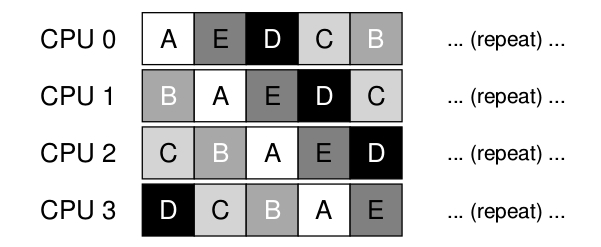
\includegraphics[width=0.7\textwidth]{ImagenesApunte/perdida_afinidad.jpg}
\end{figure}

\begin{figure}[!htb]
    \centering
    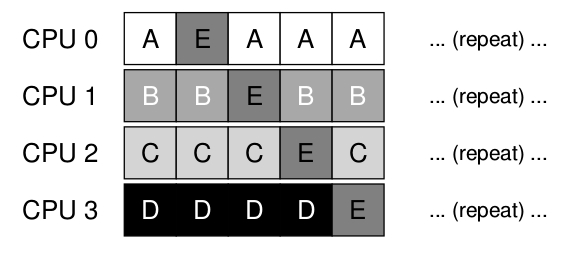
\includegraphics[width=0.7\textwidth]{ImagenesApunte/afinidad2.jpg}
\end{figure}


\subsubsection*{Multi-Queue planification}

Llamada Multi-Queue Multiprocessor Scheduling (MQMS), agrega múltiples colas, donde cada cola sigue una determinada disciplina de planificación. Este sistema es completamente escalable, a medida que crecen las CPUs, crecen las colas, sacando del problema los bloqueos y los caches. Otra ventaja que tiene es que provee afinidad de cache intrínsecamente, las tareas intentan mantenerse en la CPU en la que fueron planificadas.

El problema que presenta es el desbalance de ejecución (load imbalance). Esto sucede cuando un CPU esta sobrecargada de procesos mientras que otra no hace nada, llevando a un mayor desgaste al primero. Una solución seria moviendo las tareas de un CPU a otro, técnica llamada \emph{migration}.

\begin{figure}[!htb]
    \centering
    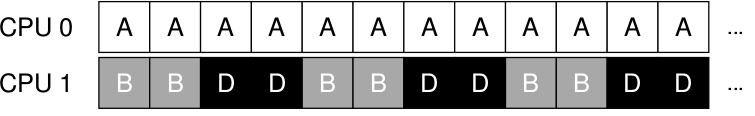
\includegraphics[width=0.7\textwidth]{ImagenesApunte/load_imbalance.jpg}
    \caption{Desbalance de ejecución.}
\end{figure}

\subsection*{El planificador de Linux: Completly Fair Scheduler}
Este planificador introdujo un algoritmo que calculaba en tiempo constante el time-slice y las colas de ejecución por proceso. Introdujo el concepto de Rotating Staircase Deadline Scheduler, que lleva al concepto de fair-share scheduler.

Una característica importante de este Completly Fair Scheduler (CFS) es que no otorga un determinado time-slice a un proceso, si no que le otorga una proporción del procesador, dependiente de la carga del sistema. 

Para poder ser eficiente, CFS intenta gastar poco tiempo tomando decisiones de planificación. Esto lo consigue gracias a su diseño y al uso inteligente de las estructuras de datos.

\subsubsection*{Funcionamiento}
Mientras que los planificadores tradicionales otorgan un time-slice fijo, CFS divide el tiempo del procesador entre los procesos que están compitiendo por ella. Esto lo hace mediante una técnica llamada virtual runtime (Vruntime). El vruntime es el runtime que corrió cada proceso normalizado por el numero de procesos runnable (medido en nanosegundos).

A medida que un proceso se ejecuta acumula vruntime, y al momento de decidir cual correr, CFS selecciona al proceso que menos vruntime tiene. Esto tiene dos cuestiones clave:
\begin{itemize}
    \item Si CFS cambia de proceso en tiempos muy pequeños estará garantizando que todos los procesos se ejecuten a costa de perdida de performance debido a la cantidad de context switches. 
    \item Si CFS cambia pocas veces, la performance del scheduler es buena, pero el costo esta puesto del lado de la equidad entre procesos (fairness).
\end{itemize}

\textit{En un estudio realizado por Google en uno de sus servidores encontró que incluso después de varias optimizaciones, el tiempo de planificación uso el 5$\%$ del tiempo.}

\medskip

El CFS se maneja entre estos valores mediante varios parámetros.
\begin{itemize}
    \item \textbf{sched\_latency}: Determina cuanto tiempo un proceso tiene que ejecutarse antes de considerar un switch. (time slice dinámico) Un valor común es 48ms, este es dividido entre todos los procesos ejecutándose en la CPU. CFS va a ser completamente justo con todos. Claramente el problema acá surge si hay muchos procesos, el time-slice seria muy pequeño, para eso esta el siguiente parámetro.
    
    \item \textbf{min\_granularity}: Establece un valor mínimo del time-slice, asegurándose que nadie tenga menos de este tiempo de ejecución y de que no haya un overhead por el context switch. Normalmente 6ms.
\end{itemize}

El CFS tiene una interrupción periódica de tiempo cada 1ms, para que pueda tomar decisiones.

\subsubsection*{Prioridades: Weighting - Niceness}
Algo que tiene el CFS es que se pueden asignar prioridades sobre los procesos por parte del usuario y administrador. El valor va de -20 a +19. El valor por defecto es 0, el que mas prioridad tiene es -20, y el que menos tiene es +19.

\begin{minted}{C}
    static const int prio_to_weight[40] = {
    /* -20 */    88761,   71755,  56483,  46273,  36291,
    /* -15 */    29154,   23254,  18705,  14949,  11916,
    /* -10 */     9548,    7620,   6100,   4904,   3906,
    /* -5 */      3121,    2501,   1991,   1586,   1277,
    /*  0 */      1024,     820,    655,    526,   423,
    /*  5 */       335,     272,    215,    172,   137,
    /* 10 */       110,      87,     70,     56,   45,
    /* 15 */        36,      29,     23,     18,   15, /* 0 */
    };
\end{minted}

Para obtener el time slice queda de la forma:
\begin{center}
    \begin{math}
        time\_slice_{k} = \frac{weight_{k}}{\sum^{n-1}_{i=0}weight_{i}} \cdot sched\_latency
    \end{math}  
\end{center}

\begin{center}
    \begin{math}
        vrntime_{i} = vrntime_{i} + \frac{weight_{0}}{weight_{i}} \cdot runtime_{i}
    \end{math}  
\end{center}

\subsubsection*{Arboles Rojo-Negro}
Para que el sistema sea eficiente, se utiliza esta estructura, ya que sus tiempos son muy buenos, O(log(n))

\begin{figure}[!htb]
    \centering
    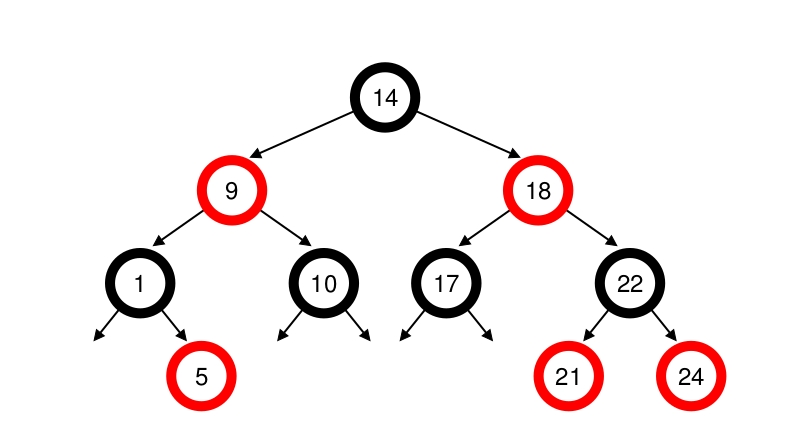
\includegraphics[width=0.7\textwidth]{ImagenesApunte/arbolRojoNegro.jpg}
\end{figure}

El algoritmo es el siguiente:
\begin{enumerate}
    \item El nodo mas a la izquierda del árbol es el elegido, ya que es el que menos tiempo se ejecuto.
    \item Si el proceso termina, se elimina del árbol.
    \item Si el proceso alcanza su máximo tiempo de ejecución o para su ejecución voluntariamente, se reinserta en el árbol basado en su nuevo tiempo.
    \item Repetir para el nuevo nodo mas a la izquierda.
\end{enumerate}

\subsubsection*{API}
\begin{itemize}
    \item nice(): establece un valor de niceness.
    \item sched\_yield(): permite a un proceso ceder el uso de la CPU.
\end{itemize}

\subsubsection*{unix Xv6}
El enfoque que utilizan los sistemas operativos para crear la ilusión de que cada proceso tiene su propio procesador virtual es mediante la multiplexación de los procesos sobre el hardware disponible.

Xv6 multiplexa cambiando en cada procesador un proceso por otro en dos ocasiones:
\begin{itemize}
    \item Los mecanismos de xv6 sleep y wakeup cambian cuando un proceso espera que se complete una operación de I/O, cuando espera por la finalización de un proceso hijo (wait) o cuando el proceso espera en la system call sleep().
    \item Xv6 periódicamente fuerza un cambio cuando un proceso de usuario se está ejecutando
\end{itemize}

Esto crea la ilusión de que cada proceso tiene su propia CPU, entre otras cosas. Este cambio entre procesos se traduce en un cambio entre modo usuario - modo kernel - modo usuario .

\begin{minted}{C}
      // Per−CPU process scheduler.
      // Each CPU calls scheduler() after setting itself up.
      // Scheduler never returns. It loops, doing:
      // − choose a process to run
      // − switch to start running that process
      // − eventually that process transfers control
      // via swtch back to the scheduler.
      void
      scheduler(void)
      {
        struct proc *p;
        struct cpu *c = mycpu();
        c->proc = 0;
    
        for(;;){
            // Enable interrupts on this processor.
            sti();
        
            // Loop over process table looking for process to run.
            acquire(&ptable.lock);
            for(p = ptable.proc; p < &ptable.proc[NPROC]; p++){
                if(p->state != RUNNABLE)
                    continue;
                
                // Switch to chosen process. It is the process’s job
                // to release ptable.lock and then reacquire it
                // before jumping back to us.
                c->proc = p;
                switchuvm(p);
                p->state = RUNNING;
                
                swtch(&(c->scheduler), p->context);
                switchkvm();
                
                // Process is done running for now.
                // It should have changed its p−>state before coming back.
                c->proc = 0;
            }
            release(&ptable.lock);
        }
    }
\end{minted}

% decir como lo logra, por que, que devuelve en las preguntas

% usar los type def de los tipos, dan mas sentido semantico a las lineas que poner int directamente

% CR3 es el registro que tiene la direccion fisica del comienzo de la tabla (lo tiene la MMU)

% pgdir_walk() toma un comienzo de una pg directory (direccion virtual), create es un bool, devuelve un puntero al lugar donde se encuentra la traduccion de la direccion virtual (NO EL CONTENIDO DEL CASILLERO, UN PUNTERO AL MISMO) casillero dentro de la tabla donde esta la traduccion - puntero al segundo PGNUM
% si no existe la tabla, y create = true, se crea esa tabla y se devuelve el correspondiente lugar (pmap.c)
% ver los macros PAGE TO PA y esas
% page_lookup: devuelve un puntero a un struct (direccion fisica) - create = 0, no debe de modificar nada - pte_store es para guardar informacion de lo que habia en el casillero de la tabla, si no es null guardo lo que me da pg_walk? Si
% page_insert: recorrer la estructura de 2 niveles con pg_walk -> nos da el puntero al casillero que tenemos que rellenar - pensar que se le pasa a create (1? -  No pensar como un caso particular si ya existe algo mapeado!!!! Afecta para mas adelante, ver como se organiza el codigo, que pasos seguir, viendo donde colocar ppref es la clave del manejo de ese caso - la parte de invalidar la TLB se puede hacer en page_remove() -
% page_remove: llama a page_lookup(), con el tercer argumento ver como settear a 0 el contenido del mapeo anterior
% no hay relacion entre el arreglo y el arreglo de las paginas fisicas las cuales reprenta

% soportar paginas grandes (de mas de 4KB de una) me hago un bypass de todas las paginas intermedias, mapeo una directa mas grande a memoria (son 4MB), se acceden directamente a estas paginas - 22 bits de offset (le agrega el indice de la pagina en la que no esta) - la MMU tiene un bit especial para indicarlo, si esta en 1 mapea a 4MB. Se activan con un registro CR4 (lo hacemos nosotros)
% boot_map_region (con 4kb solamente) - no debe incrementar el contador de referencias de las paginas

% usando el page directory primitivo (antes de la parte 3), solo podemos acceder a 4MB
% al pedir memoria en boot alloc que no me pase de esos 4mb mapeados

% si se desreferencia NULL en el kernel (de jos), esto hace que se reinicie continuamente

% KADDR(PTE_ADDR(pgdir[index1])) desreferencio un puntero virtual

% tenemos espacio para 256mb en jos

% boot.S, el comienzo de todo (el bootloader) (otra parte esta despues en C - main.c)
% Pasa de modo protegido a modo real
% Llamada a bootmain, es una funcion en C que continua con la ejecucion del bootloader -> Esta en main.c
% bootmain lee del disco, para traer el kernel que NO esta en memoria todavia (readseg)
% Se lee el header y se va trayendo las partes de binario 
% Al final se hace la llamada a funcion realizando casteos (el entry point desde el ELF header) (es una direccion de memoria directamente) -> salta a kern/entry.S 'nombre' entry
% El binario ELF donde esta se puede ver con 'readelf -a obj/kern/kernel (| less)'
% entry.S ya es el kernel, es el inicio de su ejecucion, activa la paginacion, poniendo en cr3 la entrada a la tabla de directorios
% mueve la direccion de 'relocated' a un registro, y despues salta al valor del registro.
% al instruction pointer no le cambia en nada la paginacion, pero al activarla (todos los simbolos del kernel fueron compilados en direcciones altas) necesitamos saltar
% el ip tenia una direccion baja, despues del jump el ip va a ser el mismo pero con una F adelante
% los primeros 4mb virtuales mapean a los primeros 4mb fisicos
% setea el frame pointer inicial en 0 (para el backtrace)
% despues va a i386_init() en init.c


%%%%%%%%% TP2: procesos en JOS
% Combinar codigo esqueleto a nuestro codigo creando 2 ramas nuevas, entrega y base (ambas con nuestro codigo)
% make grade para probar que esta finalmente
% Crear nocion de proceso -> Se llaman environments en JOS
% Ejecucion de un unico proceso, lo crea y manda a ejecutar, Soporte para syscalls
% El proceso es el struct Env: sus ids
% EnvType: va a haber mas de un tipo de proceso en jos mas adelante
% env_status: ENV_FREE(representa que esta en el arreglo de procesos libres), ENV_RUNNABLE(no estoy en cpu, pero estoy listo para ir a correr), ENV_NOT_RUNNABLE(estoy bloqueado), ENV_RUNNING, ENV_DYING(estado opcional, ocurre cuando muere un proceso que esta en otro cpu - TP3)
% env_runs: contador que dice cuantas veces fue alocado el proceso en el cpu
% el page directory table de cada proceso
% struct Trapframe: Es la representacion del estado del CPU en un estado del tiempo
% *env_link: va a permitir formar una lista de procesos
% Process Control Block: el arreglo envs contiene todos los procesos. Se tiene una lista env_free_list de los procesos libres tambien. Mismo sistema que para el arreglo de struct pages
% #define NENV define cuantos procesos va a soportar
% no es que existe esta cantidad de procesos, es que se reservo memoria para esta cantiad de procesos. Para que corran los guardo en estos lugares.
% curenv: variable que mantiene una referencia al proceso que se esta ejecutando ahora en el cpu
% el arreglo nuevo este se pondria usando el mismo mecanismo que para pages (boot_alloc)
%%%%%%
% REGISTROS EN x86
% Segment registers: cs(code segment)(CPL - muestra el nivel de privilegio que tiene el proceso en el cpu - Los Rings- Current Privilege Level - para cambiarlo hay que estar en modo kernel, cambiar este valor lleva a modo usuario)(una vez que pase a modo usuario, como vuelvo? No tengo provilegios),ds(data segment),es,ss -> controlan la segmentacion, protengen la memoria
% General: edi,esi,ebp,ebx,edx,ecx,eax
% Special: esp,eip,eflags(como el de estructura)(overflow, negativo, ...)(hay que mantener los flags en cada context switch)
% Control: cr0,cr1,cre2,cr3,gdtr,... (activan o desactivan opciones del cpu) (son globales al comportamiento del cpu, no dependen del proceso)
% Segmentacion en x86: nos llega una direccion lineal a la paginacion
% divide a la memoria en segmentos , dependiendo de lo que queramos acceder, elegimos un segmento
% Hay una tabla descriptores de segmento, el descriptor de segmento se elige con el registro de segmento
% los registros de segmentos tienen una parte que dice con que permisos intentan acceder (Requested Privilege Level)
% permisos, 0 kernel, 3 cualquiera
% Cuidado con las flechas, puso valores al reves!!!!!!!!!!!!!!!!!!!!!!! en la diapo segmentacion en x86 con tablas y un cubo
% todos los segmentos tienen direccion base 0x0 y limite 4gb
% LA VIRTUAL ADDRESS SIEMPRE VA A SER IGUAL A LA LINEAR ADDRESS
% macro SEG - observar - configura segmentos
% boot loader configura una tabla de segmentacion para pasar de modo real a modo protegido.
% en env.c se define la tabla ?gdt? (como pmap.c)
%%%%% TAREA 1 
% mem_init_envs() usamos boot alocc para reservar la memoria - NENV lugares a reservar - abajo del lugar de pages en el mapeo, de la misma forma que en pages - solo lectura este lugar
% env_init() - inicializar el arreglo envs - setear estado en FREE - armar la lista enlazada - en principio todo libre - algo esta corriendo? No existe ningun proceso creado, todo esta free - el kernel no se cuenta a si mismo como un proceso!!!!! Linux se incluye, jos no, diseño
% env_alloc() inspeccionar 
% el id del proceso no es ir sumando uno, estan relacionados con la region de memoria - la busqueda en envid2env es O(1)
% env_setup_vm() configura el page directory del environment - se usa una copia del page directory del kernel - NO se modifica cr3 - copia del kernel
%%%%% TAREA 2 - CARGA DE BINARIOS
% Armar el espacio de direcciones para cada uno de los segmentos - heap, data, code, stack - No tenemos heap, habria que implementar sbrk
% 
%
% el puntero al binario se puede castear a un struct elf y empezar a usar las cosas.
% region_alloc() llama a page_insert() para reservar memoria
% cuando hicimos region_alloc() lo hicimos en el page_directory del proceso, el cpi? tiene que ser en el del hijo - se hace cambiando el valor de cr3
% instruction pointer donde diga el elf en el entry 
%
% %%%% TAREA 3 
% iret: es ret en esteroides - espera un onton de cosas - hace un monton de cosas a la vez - circuito especial - hace un cambio de contexto
% ret lee el tope del stack, y lo pone en el instruction pointer y salta
% no tiene que modificar x cosa
% env_pop_tf no retorna nunca, vamos a modo usuario, por eso se da el lujo de destruir el stack pointer salteando posiciones sumando 8
% hacer seguimiendo con gdb
% va a fallar cuando intenemos hacer la syscall (imprimir a pantalla) (qemu se va a reiniciar) (general protection fault)
%
%%%%%% TAREA 4
% IDT y Syscalls en JOS
% 
% Interrupciones y Excepciones
% interrupciones: son generadas debido a señales externas de dispositivos de hardware o ejecutadas por software (ej breakpoint)
% excepciones: ocurren cuando el CPU detecta un error en la ejecucion de una instruccion, son unicas, ej division por 0, la alu no puede manejar eso y tira la excepcion. Ej segmentation fault, el programa quiere acceder a una region donde no tiene permisos
% los hexagonos(ppt) simbolizan por  donde se entra/sale a/del kernel
% en el lado del kernel hay handlers en la IDT - interrupt descriptor table - Intel Vol 3A - C-6.10
% IDT Limit es el tamaño de la tabla
% Trap gates (excepciones) istrap = 1
% interrupt gates istrap = 0
% se deben de poder manejar excepciones en el medio de excepciones, se tienen que anidar - Intel Vol 3A - C-6.11
% IDT Interrupt Call Flow %%%%%%%%%%%%
% se produce un cambio de stack (se pasa de un usuario y se pasa a uno del kernel) Se obtiene a traves de este descriptor(segment descriptor?) adentro de la GDT
% se hace un push en el stak de: SS, ESP, EFLAGS, CS (code segment), EIP (instruction pointes, hay que saber a donde volver)
% si la excepcion genero un codigo de error se realiza otro push  (Error code: yes) (se pushea el error code)
% tabla de excepciones  Intel Vol 3A - C-6.3.1
% la syscall esta entre las 32-255 interrupciones (son user defined)
% trap.c idt_pd tiene base y limit, hay una funcion helper que traduce del numero al nombre - es un struct que se hizo para poder poner en el formato que se espera el registro del cpu (idtr) (47 idt_base_address 16|15 idt_limit 0)
% trap_init()
% configurar la idt hacer con unas macros llamadas SETGATE(idt[0], numero excepc/interrump, flags..., handler_0)
% asi con todas - handler_0 es un puntero a la funcion que maneja esa interrupcion - desde donde se va a ejecutar el handler ?SIMILAR A GD_KD? (para sel)
% off es handler_0 (ver consigna por convencion nombres)
% dpl - nivel requerido de privilegios para ejecutar el handler - modo usuario para syscall (3) desde donde quiero ejecutar esta interrupcion
% T_DIVIDE nivel de privilegio 0, solo desde el kernel (dpl)
% SETGATE(idt[0], numero excepc/interrump, flags..., handler_0)
% SETGATE(idt[1], numero excepc/interrump, flags..., handler_1)
% SETGATE(idt[2], numero excepc/interrump, flags..., handler_2)
% SETGATE(idt[3], numero excepc/interrump, flags..., handler_3)
% REVISAR HASTA DONDE
% usar unas macros que ya tienen esa definicion (inc/trap.h) !!!!!!!!!!!!!!!!!!!!
% hay constantes que definen el nombre - T_DIVIDE / T_DEBUG / ...
% setear correctamente istrap segun corresponda
% trap_init_percpu
% TSS : task segment selector
% GD_KD : global descriptor del kernel
% 
% gatedesc tiene cada una de las entradas de esta tabla
%
% en inc/mmu.h esta struct Gatedesc, se le dice cuantos bits miden
% de donde salen los handler?  las tenemos que hacer -> codigo assembly -> TRAPHANDLER  name - > handler_0 - .globl declara una funcion
% donde? kern/trapentry.S
% TRAPHANDLER(_NOEC) (name,num)
% TRAPHANDLER_NOEC(handler_0,T_DIVIDE)
% PARA LAS SYSCALLS CON _NOEC no hay porque pushear un error code
% 
% _alltraps:
% es el codigo comun para cualquier interrupcion, entra en juego la forma que tiene el stack, y finalmente la forma que se tiene que llamar a codigo C
% Ej bootloader, codigo asm puntual especifico para pasar a codigo C
% diapo del stack, faltan guardar todos los demas de la convencion de llamadas de funciones, %eax,%ebx,... todos los que se estaban usando en modo usuario
% leer 1213 del push
% push %ds/%es // pisar los registros tambien, linea 1219
% push de eax, de ebx, ... // pushal
% necesitamos un puntero, push %esp
% call trap     //funcion en C a la cual llegan todas las interrupciones // al final de esa funcion con env_run hace la vuelta al usuario que hace pop_frame que restaura registros
% recibe un struct Trapframe* -> (en inc/trap.h)  tiene los registros de proposito gral, es, data segment, padding, trapno, err,...
% tiene el mismo layout que lo del stack, queremos replicar la estructura, parte ya fue rellenada por el cpu (desde el fondo hasta trapno)
% queremos pushear al stack trap_es, push_regs y trap_ds, asi tenemos la estructura (esto esta en _alltraps tambien) - para los registros, hay una instruccion que pushea todos juntos ->
% pushal - TIRA TODOS LOS REGISTROS AL STACK EN EL MISMO ORDEN EN QUE ESTAN DEFINIDOS!!!!!!!!!!!!!!!!!!!!!!!!!!!
%
% trap_dispath
% switch(tf->tf_trapno){
% case T_SYSCALL: syscall_handler(); break; ...}
%
% en alltraps pisar es y ds GD_KD -> mov %ds, $(GD_KD) es la forma de decirle al cpu algo(revisar clase para el motivo) 
%
% TAREA 5 - LA MMU ASEGURA ACCESO DIRECTO A REGIONES DE MEMORIA, pero no valida ej es del kernel
% agregar proteccion mediante software -> pmap.c -> user_mem_check(...), llamar a user_mem_assert(...)
% en sys_cputs llamar user_mem_assert(curenv,s,len,PTE_P|PTE_U|)
% en user_mem_check revisar las paginas - se puede usar pgdir_walk, pg_lookup
% if(page & (perms | PTE_P) == PTE_P|perms)...
% 
%
% evil hello %%%%%%%%%%%%%%% se puede ejecutar antes de implementar la proteccion
% se quiere imprimir el primer caracter - no nos deberia de dejar desreferenciar la direccion del kernel, no se llega a ejecutar la syscall, se muere en char first = ...
% lo rebota la mmu (proteccion que ya tenemos)

\newpage

\section*{Novena y décima clase}
\section{Concurrencia}
Definición de Thread: Un thread es una secuencia de ejecución atómica que representa una tarea planificable de ejecución.

Secuencia de ejecución atómica porque cada thread ejecuta una secuencia de instrucciones como lo hace un bloque de código en el modelo de programación secuencial (Desde el punto de vista del thread, tiene un inicio y fin y nunca para). Y tarea planificable de ejecución ya que el sistema operativo tiene injerencia sobre el mismo en cualquier momento y puede ejecutarlo, suspenderlo y continuarlo cuando él desee.

'Pretender estar haciendo varias cosas a la vez, pero siempre le dedicamos el tiempo de procesamiento a una cosa.' Es distinto a la ejecución paralela, en ese caso si se hacen a la vez, en el mismo tiempo t.


\begin{minted}{C}
    {
    instruccion1
    instruccion2
    instruccion3
    instruccion4
    ...
    instruccionN
    }
\end{minted}
\begin{center}\textit{Como se vería un thread: 'secuencia independiente de instrucciones que representa una tarea planificable de ejecución'.}\end{center}

\begin{figure}[!htb]
    \centering
    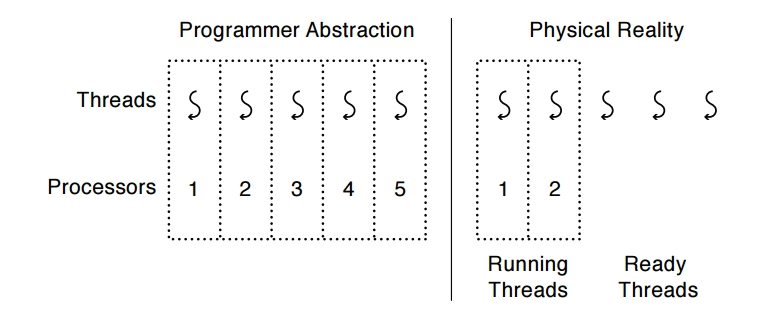
\includegraphics[width=0.7\textwidth]{ImagenesApunte/threads_abstraction.jpg}
\end{figure}

\subsection*{Threads vs procesos}

Un proceso es un \emph{programa} en ejecución con derechos restringidos, mientras que un thread es una secuencia independiente de instrucciones ejecutándose dentro de un programa.

\subsection*{Threads}
Los threads cuentan con las siguientes características:
\begin{itemize}
    \item Thread ID
    \item Un conjunto de valores de registros
    \item Un stack propio
    \item Una política y prioridad de ejecución
    \item Su propio \emph{errno}
    \item Datos específicos del thread.
\end{itemize}

Hay diferentes casos de ejecución, un Thread por proceso, muchos Threads por proceso, muchos procesos de un solo Thread, y muchos Kernel Threads (el kernel puede ejecutar varios para aprovechar recursos).

\subsubsection*{Thread Scheduler}
Ya que generalmente se trabajan con menos procesadores que Threads, es necesaria alguna forma de planificar quien se ejecuta, esta forma tiene que ser transparente, el programador no debe preocuparse de cuando es suspendido o no el thread. Esto hace que los Threads provean de un modelo de ejecución en el cual cada thread corre en un procesador virtual dedicado (exclusivo) con una velocidad variable e impredecible. (No podemos decir con que velocidad y cuando se va a ejecutar.)

Desde el punto de vista del thread cada instrucción se ejecuta inmediatamente una detrás de otra (atómico). Pero el que decide cuando se ejecuta es el planificador de threads o thread scheduler. El thread piensa que nunca paro de ejecutarse. Los mismos pueden ser ejecutados de 2 formas, de forma cooperativa (no hay interrupción a menos que se solicite) y forma preemptiva (un thread en estado running puede ser movido en cualquier momento).

\begin{figure}[!htb]
    \centering
    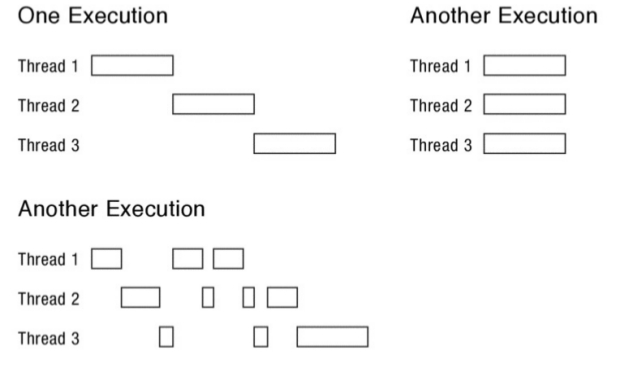
\includegraphics[width=0.7\textwidth]{ImagenesApunte/threads_execution.jpg}
\end{figure}

\subsubsection*{La API}
Tienen una biblioteca, no forma parte de la entandar.

Principalmente los threads se deben de poder crear y hacer join (esperar a que termine otro thread).

Un ejemplo utilizando la biblioteca \emph{pthread}.
\begin{minted}{C}
    #include<stdio.h>
    #include<pthread.h>
    #include<assert.h>
    #include<stdlib.h>
    
    
    typedef struct __myarg_t {
        int a;
        int b;
    } myarg_t;
    
    
    typedef struct __myret_t {
        int x;
        int y;
    } myret_t;
    
    void *mythread(void *arg) {
        myarg_t *m = (myarg_t *) arg;
        printf("%d %d\n", m->a, m->b);
        myret_t *r = malloc(sizeof(myret_t));
        r->x = 1;
        r->y = 2;
        return (void *) r;
    }
    
    int main(int argc, char *argv[]) {
        int rc;
        pthread_t p;
        myret_t *m;
        myarg_t args;
    
        args.a = 10;
        args.b = 20;
        pthread_create(&p, NULL, mythread, &args);
        pthread_join(p, (void **) &m);
        printf("returned %d %d\n", m->x, m->y);
        free(m);
        return 0;
    }
\end{minted}

\subsubsection*{¿Por que se usan los threads?}
\begin{itemize}
    \item Paralelismo: Se tiene el potencial de acelerar el rendimiento del programa.
    \item Si un thread realiza I/O, otro thread podría realizar otras operaciones mientras este listo para correr.
\end{itemize}

\subsubsection*{¿Por que se complica con los recursos compartidos?}
Porque no hay sincronización entre los threads. Corren de forma diferente dependiendo de lo que decida el planificador.


\subsubsection*{Estado Per-Thread y Threads Control Block (TCB)}
Cada thread debe tener una estructura que represente su estado. Esta estructura se denomina Thread Control Block (TCB), se crea una entrada por cada thread. La TCB almacena el estado per-thread de un thread. Este bloque debe almacenar el puntero al stack del thread y una copia de los registros en el procesador. De esta forma el sistema operativo puede crear, parar, y volver a iniciar múltiples threads sin problemas de estado de cada uno.

Por cada thread se guarda información del mismo también, ID, prioridad del planificador, y el estado.

De forma compartida se debe guardar también información, el código, variables globales, variables del heap. Todos los threads verían esta información.

\begin{figure}[!htb]
    \centering
    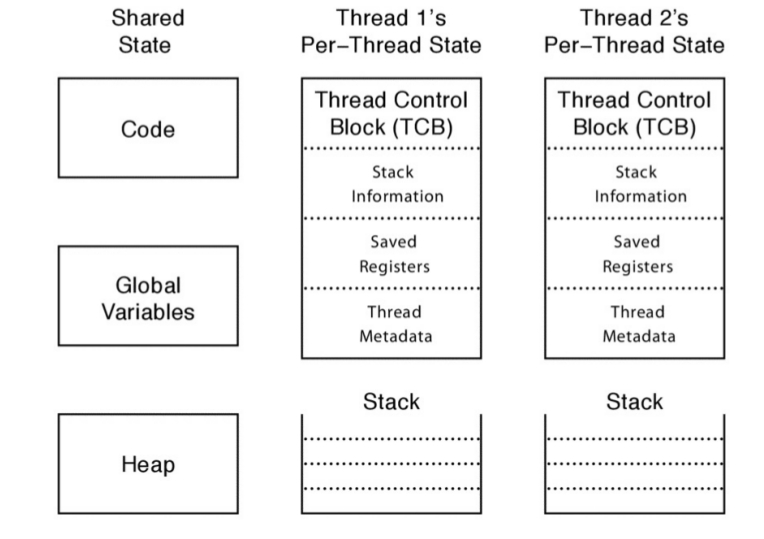
\includegraphics[width=0.7\textwidth]{ImagenesApunte/threads_data.jpg}
\end{figure}

\subsubsection*{Estados de un thread}
\begin{itemize}
    \item INIT: sucede mientras se está inicializando el estado per-thread y se está reservando el espacio de memoria necesario para estas estructuras. Una vez hecho, se setea en READY y se lo pone en una lista llamada \emph{ready list} en la cual esperan todos los threads listos para ejecutarse.
    \item READY: Indica que el thread esta listo para ser ejecutado. La TCB esta en la \emph{ready list} y los valores de los registros están en la TCB. Puede transicionar a RUNNING.
    \item RUNNING: El thread esta siendo ejecutado en este mismo instante por el procesador. Los valores de los registros están en el procesador. Puede pasar a READY si lo desalojan o preemption del mismo, o si el thread deja la ejecucion (con thread\_yield).
    \item WAITING: El thread esta esperando que algun evento suceda. No puede pasar a RUNNING directamente. Se almacena en la \emph{Waiting list}. Cuando ocurra el evento, el planificador lo pasa a estado RUNNING.
    \item FINISHED: El thread termino, no vuelve a ejecutarse. Pasa a la lista \emph{finnished list} en la que están los TCB de los threads que terminaron.
\end{itemize}

\begin{figure}[!htb]
    \centering
    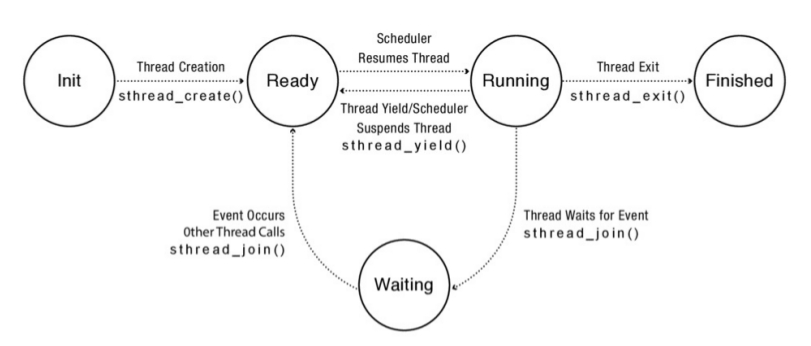
\includegraphics[width=0.8\textwidth]{ImagenesApunte/threads_estados_ejecucion.jpg}
\end{figure}

\subsection*{Diferencias con los procesos}
\begin{itemize}
    \item Los threads
        \begin{itemize}
        \item Por defecto comparten memoria
        \item Por defecto comparten los descriptores de archivos
        \item Por defecto comparten el contexto del filsystem
        \item Por defecto comparten el manejo de señales
        \end{itemize}
    \item Los Procesos
        \begin{itemize}
        \item Por defecto no comparten memoria
        \item Por defecto no comparten los descriptores de archivos
        \item Por defecto no comparten el contexto del filsystem
        \item Por defecto no comparten el manejo de señales
        \end{itemize}
\end{itemize}

Linux utiliza un modelo 1-1 (proceso-thread) con lo cual para el kernel de Linux, un thread y un proceso son lo mismo, todo es una tarea ejecutándose. (No es así en todos los sistemas operativos). El scheduler es el mismo de procesos (sabe distinguir entre los tipos solamente).

\subsection*{System Call: clone()}

La creación de un proceso y un thread llaman de fondo a esta system call (clone). Lo que las diferencia son los flags que le mandan.
\begin{minted}{C}
    #define _GNU_SOURCE
    #include <sched.h>
    
    int __clone(int (*fn) (void *arg), void *child_stack, int flags, void *args, ...
    /* pid_t *ptid, void *newtls, pid_t *ctid */ );
\end{minted}

\medskip

\begin{itemize}
    \item CLONE\_VM - share memory
    \item CLONE\_FILES - share file descriptors
    \item CLONE\_SIGHAND - share signal handlers
    \item CLONE\_VFORK - allow child to signal parent on exit
    \item CLONE\_PID - share PID (not implemented yet)
    \item CLONE\_FS - share filesystem
\end{itemize}

En el caso de un thread, se la llama con mas permisos, y en un proceso lo menos posible.



\subsection*{Sincronización}

Los programas con varios threads se pueden diferenciar en 2 tipos. Los que están compuestos por threads independientes que operan sobre datos separados entre si, y los que están compuestos por threads que trabajan de forma cooperativa entre si, compartiendo memoria y datos. Ambos casos tienen distintas formas de tratarse.

Hay que tener especial atención a como se programa cuando se sigue el modelo cooperativo, ya que la ejecución del programa depende de la forma en que los threads se intercalan en la ejecución, esta misma puede no ser determinística debido a decisiones del scheduler. Y además, los compiladores pueden reordenar instrucciones para mejorar la performance\footnote{Para evitarlo en C compilar con -O0}, algo que es invisible generalmente con un solo thread. Estos problemas pueden llevar a bugs que se caracterizan por ser sutiles, no deterministicos, y no reproducibles.

Para evitar esto, hay que estructurar el programa para que resulte fácil el razonamiento concurrente, y utilizar un conjunto de primitivas estándares para sincronizar el acceso a los recursos compartidos.

\subsubsection*{Race Conditions}

Una race condition se da cuando el resultado de un programa depende en como se intercalaron las operaciones de los threads que se ejecutan dentro de ese proceso. De hecho los threads juegan una carrera entre sus operaciones, y el resultado del programa depende de quién gane esa carrera.


\subsubsection*{Operaciones Atómicas}
Ocurre en algunos casos que algunas instrucciones no pueden dividirse en otras al momento del ensamblado. En estos casos se garantiza la ejecución de las mismas sin tener que intercalar ejecución.

Para los problemas de este tipo, los programas tienen que ser \textbf{seguros (safety)} (nada malo va a pasar), donde el programa nunca termina en un estado incorrecto , y 
\textbf{Liveness} (si algo va a pasar tiene que ser bueno), donde el programa eventualmente siempre está en un estado correcto.

\textit{Revisar el algoritmo de Peterson. Trata sobre la exclusión mutua, que permite a dos o mas procesos/hilos de ejecución compartir recursos sin conflictos, usando solo memoria compartida para la comunicación. Los algoritmos involucrados tienen que ser distintos entre los procesos, donde uno para y espera al otro}

Para lograr que sea atómico, un bloque se debe transformar a una sola.

\subsubsection*{Locks}
Un lock es una variable que permite la sincronización mediante la exclusión mutua, cuando un thread tiene el candado, ningún otro thread puede tenerlo.

Estos locks están asociados a determinados estados o partes de código, y requieren que el thread posea el lock para entrar en ese estado. Esto logra que solo un thread acceda a un recurso compartido a la vez, permitiendo la exclusión mutua.

Estos locks tienen dos estados, \textit{busy} o \textit{free}, empezando siempre en \textit{free}. Para usarlos, se pide acceso al lock con \textit{lock()} y se libera con \textit{unlock()}.
Para que esto funcione, la verificación y seteo del estado son operaciones atómicas. Si un thread ya tiene acceso a esa región, todos los demás threads esperan a que quede libre (es bloqueante).

Otras posibles acciones con locks son \textit{trylock() y timedlock()}.

Los locks deben asegurar la exclusión mutua, progress (si no esta en uso, alguien debe poder tomarlo), y bounded waiting (Si T quiere acceder al lock y existen varios threads en la misma situación, los demás tienen una cantidad finita (un límite) de posible accesos antes que T lo haga.)

La Sección Crítica es aquella sección del código fuente que se necesita que se ejecute en forma atómica. Para ello esta sección se encierra dentro de un lock.

El sistema operativo no puede inferir donde poner un lock en un programa.

\textit{Nota: Una implementación básica es escribiendo y leyendo de memoria (JOS implementa esta). En técnicas de programación concurrente se ven en detalle implementaciones.}

\subsubsection*{Condition variables}
En ciertas ocasiones puede ser necesario que un thread espere que cierta condición o estado se dé para que este continúe su ejecución, por ejemplo, un servidor web necesita esperar a que alguien le avise que hay una nueva petición web. Ahora mandarlo a esperar girando (spinning) en su propio lugar no es eficiente.

Una condition variable permite a un thread esperar a otro thread para tomar una accion. Son un objeto sincronizado que permiten de forma eficiente esperar por un cambio para compartir algún estado que está protegido por un lock.

Su API es \emph{wait()}(suelta al mutex, suspende la ejecucion, y vuelve a tomar el mutex cuando ocurre el signal()), \emph{signal()} (toma a un thread y lo pone en la ready list), y \emph{broadcast()} (pone a todos en la ready list). No confundir signal y wait con las system calls de UNIX.

Una condition variable se utiliza cuando algún tipo de señal tiene que suceder entre los threads, por ejemplo esperar por un cambio en un estado compartido o variable compartida, por ende un lock siempre debe proteger la actualización de dicho estado. Las condition variables o también llamados monitores están diseñadas para trabajar en concordancia con los lock.

\begin{minted}{C}
    pthread_mutex_t lock = PTHREAD_MUTEX_INITIALIZER;
    pthread_cond_t cond = PTHREAD_COND_INITIALIZER;
    
    pthread_mutex_lock(&lock);
    while (ready == 0)
        Pthread_cond_wait(&cond, &lock);
    Pthread_mutex_unlock(&lock);
\end{minted}

En otro hilo.
\begin{minted}{C}
    pthread_mutex_lock(&lock);
    ready = 1;
    pthread_mutex_unlock(&lock);
    
    pthread_cond_signal(&cond);
\end{minted}

Internamente mientras que esta esperando, utiliza la operación NOP.


\subsubsection*{Ejemplo en tipos de datos sincronizados}
Algunos ejemplos posibles son, una cola o un contador. Ejemplo sacado del Arpaci.
\begin{minted}{C}
    typedef struct __counter_t {
        int value;
        pthread_mutex_t lock;
    } counter_t;
    
    void init(counter_t *c) {
        c->value = 0;
        pthread_mutex_init(&c->lock, NULL);
    }
    
    
    void increment(counter_t *c) {
        pthread_mutex_lock(&c->lock);
        c->value++;
    Pthread_mutex_unlock(&c->lock);
    }
    
    void decrement(counter_t *c) {
        pthread_mutex_lock(&c->lock);
        c->value--;
        pthread_mutex_unlock(&c->lock);
    }
    
    int get(counter_t *c) {
        pthread_mutex_lock(&c->lock);
        int rc = c->value;
        pthread_mutex_unlock(&c->lock);
        return rc;
    }
\end{minted}

\subsection*{Errores comunes en concurrencia}

\subsubsection*{Non Deadlocks}
\begin{itemize}
    \item Atomicity violation: “el deseo de la serialización entre múltiples accesos a memoria es violado”.
    \item Order Violation: “El orden deseado entre accesos a memoria se ha cambiado”
\end{itemize}

\subsubsection*{Deadlocks}
Ocurre cuando dos o mas threads se bloquean entre si. Se puede dar cuando uno obtiene el lock, y por algun motivo nunca lo libera (exclusión mutua). Hold and wait, un thread mantiene un recurso reservado para si mismo mientras espera que se de alguna condición. No preemption, los recursos adquiridos no pueden ser desalojados por la fuerza (preempted). Circular wait, un conjunto de threads que de forma circular cada uno reserva recursos que necesita otro thread.

La circular wait se previene escribiendo código que nunca induzca a esperas circulares, por ejemplo con el establecimiento de un orden total, este orden asegurará que no se caiga en espera circular.

El hold and wait se previene haciendo que los lock se tomen en forma atómica:

% TP3 
% resolver conflictos en el merge, sacar de entrega_tp2
% los procesos estan mapeados al final del kernel hasta ahora
% a traves de la libreria estandar, (umain) se encarga de devolver el control a JOS
% agregar soporte para multiples procesos
% implementamos Symmetric Multi Processing - todos los cpus son iguales en caunto recursos, su propio set de registros, propia cache, todos arrancan en modo real, su propio controlador de 
% interrupciones
% Todos comparten el acceso a memoria (MMU y bus de datos)
% Cada procesador tiene su propio registro del stack pointer (pero apuntan a memoria, cada uno tiene su region)
% Todos iguales excepto en el arranque
% Empiezan dormidos, y hay que prenderlos (el bootstrap processor) - lo hace con interrupciones  - BPS
% El BPS detecta en inicializa los APs (application processors) usando LAPIC - pone el IP en el mismo punto para salir del modo real,pasar a modo protegido , inicializar paginado
% hay que diferenciar el BPS de los APs, no queremos que sigan los mismos pasos (ejecutarian lo mismo) - la inicialiazacion es desde otro lado
% PIC (programmable interrup controller) - mapea señales del bus de interrupciones a interrupts del procesador - lo hace segun IRQ base + offset - IRQ N -> PIC -> INT N -> CPU (con un solo cpu)
% evoluciona a APIC (mas cpus) - hay de entrada salida (con dispositivos) y los local APIC que estan adentro del cpu (manejan interrupciones internas a dispositivos del cpu)
% todos se comunican a traves del mismo bus de interrupciones - permiten comunicacion entre cpus
% por compatibilidad hay un PIC afuera tambien - el pic configura al apic, lo inicia
% el BPS configura PIC y LAPIC
% LAPIC mapeado a direcciones fisicas altas - lapic_init() - similar ocurre con el PIC del BPS en pic_init()
% no hay que mapearlo normalmenmte (esta en un lugar de i/o) - hay que usar flags especiales para decir que es MMIO - CACHE DISABLE (PTE_CD) y WRITE THROUGH (PTE_WT)
% los PAS arrancan en memoria fisica baja - hay que inicializar cada stacj para cada cpu
% struct Taskstate dice que stack usar en la ejecucion - reserva una pagina para mantener el stack del cpu (en el archivo de la funcion mpconfig se ve todo esto)
% volatile - le dice al compilador que no la optimice - cada lectura y escritura tiene un sentido, por mas que parezca que no
% APS empiezan en mpentry.S, quedan idle
% variable SPIN_LOCK para tener mas info debuggeando
% TAREA 0
% regiones de memoria invalida para protegerse - mem_init_mp() mapea estas regiones para cada cpu - pagina 7 como ocupada - copia el codigo - la variable esta en memoria, en algun momento va a cambiar
% marcar pag 7 como ocupada
% TAREA 3
% sesion gdb
%% TAREA 1
%
% SCHEDULER JOS
% el mas simple, usamos round robin - recorre uno por uno los procesos y si alguno esta listo lo pone a ejecutar - si no hay se pone a dormir
% 2 fases - uno sin desalojo - despues se hace otro que le agrega desalojo con timeslices
% funcion sched_yield()
% variable thiscpu que devuelve siempre en que cpu esta corriendo - macro curenv
%
% funcion hlt - pone a dormir hasta que llega una interrupcion - estado de consumo de energia minimo
% habilitar flag de interrupciones para el usuario en env_create -> en eflags - FL_IF
% hay un reloj al lado del cpu, lo configuramos para que nos envie interrupciones de forma periodica - le llega al apic
%
%
% %%%%%%%%%%%%%%%%%%%%%%%%%%%%%% IPC - COMUNICACION ENTRE PROCESOS - TAREA 4
% solo el kernel puede permitir que los procesos se comuniquen
% formas comunicar: pipes- fifos-colas de mensajes-señales-memoria compartida
% para sincronizar: file locks - semaforos
%
% en JOS implementamos memoria compartida (la mas facil desde el kernel - no tiene que hacer nada - mapea una misma pagina a dos procesos)
% el RECEPTOR declara que quiere una pagina, y donde
% el TRANSMISOR declara que quiere enviar una pagina y cual
% se transmite un unico valor entero
% tener cuidado con los permisos, nunca dar mas de los que ya tenia
% el kernel se da cuenta con syscalls que se quieren comunicar
% las operaciones terminan exitosamente, o no terminan nunca (recibir, ninguno envia)
% 
% %%%% 2 syscalls
% ipc_recv y ipc_send (wrappers de la syscall) son asimetricas (una se bloquea, la otra no)
% si alguien esta recibiendo, hago el mapeo, si no hay nadie, devuelve que fallo(el send)
% la pagina ya esta alocada en el proceso que envia
% puede fallar por permisos (no puedo dar lectura/escritura a alguien si no tengo lectura/escritura)
% struct Env tiene mas campos (metadata)
% ipc_try_send (queda loopeando la libreria de JOS)
%
% %%%%%%%%%%%%%%%%%%%%%%%%%%%%% FORK 
% jos exokernel, desde el kernel lo minimo necesario, lo demas del lado del usuario 
% sys_exofork() (estado del cpu, pid a devolver, estado del nuevo proceso) - kernel ------------------ user - fork (copia address space)
% varias sysacall llamadas desde fork (nivel usuario)
%
% %%%%% evid2env 
% checkeo de permisos, se usa en las syscalls
%
% %%%%%%%% dumbfork - protoversion, programa de usuario, aproximacion de como deberian imlementarse la funciond de usuario fork
% %%%% fork_v0: de 0 a UTOP - dup_or_share
%
% entry.S se establecen variables globales con la relacion, UENVS - UPAGES - UVPT (esta en meminit) inserta recursivamente en su page directory su page directory? interpretar como un arreglo de las paginas fisicas reales de 4k
%
% %%%%%%%% fork COW (mas eficiente que el otro fork, con exec pisabamos todo lo que copiamos) TAREA 6
% genera copias de plas paginas solo cuando es necesario -> en una escritura
% por cada pagina a copiar en el proceso hijo, lo unico que se hace es generar el mapping de la pagina fisica y marcarlo como COW(bit especial)
% se hacen checkeos a medida que se necesitan - es super optimo - excelente por si viene un exec
% cuando se vaya a escribir, se detecta y se hace la transferencia de datos
% el usuario no se entera, es transparente
% las lecturas se mantienten
% las escrituras se transforman a COW - marcar como COW hijo y padre! por que es necesario marcar ambos????????? uno en principio no sabe que proceso vuelve a correr primero (padre o hijo), que pasa si uno escribe antes que el otro
% escritura -> page fault por no tener el bit, nos fijamos el COW tambien
% %%%%%%%%%%%%%%%%%%%%% TAREA 5
% set_pgfault_handler - reserva memoria para la pila de excepciones e instala el manejador del kernel
% pgfault_upcall - handler que siempre se instala en el userspace - en el kernel se registra el de assembly
% 
% seteo del struct UTrapframe
% curenv->tf.tf_eip = curenv->env_pgfault_upcall
% curenv->tf.tf_esp = USTACKTOP
% env_run(curenv)
%
% sigue en pfentry.S - instruccion final ret (necesitamos un instruction pointer antes)- reorganizacion del stack para dejarlo como si alguien hubiera llamado a esta funcion
% mirar trap.c - se deja de espacio una extra word que es clave % |eip|<-esp(apunta aca)
% esp_a_colver = *(esp+offset)
% *(esp_a_volver - 4) = eip
%
% mover eip a algun lado (instruccion extra para que este apuntando a PushRegs)
% popal
% una instruccion para poder hacer la siguiente, que apunte a eflags
% popfl (restaura flags)
% configurar stack pointer
% popl %esp
% ret
%
%
% sys_set_pgfault_handler(_pgfault_upcall) [en set_pgfault_handler] pgfault.c - llama a la funcion de asm - adentro del if
% fork() - set_page_fault_handler
%
% en el fork NO mapear la region reservada de la pila de excepciones!!!!!!!!!!!! no se puede producir una pagefault en este lugar, si se mapea podrian pasar.
% duppage NO llama a sys_page_alloc

\newpage

\section*{Undécima clase}
\section{Sistema de archivos}
Un sistema de archivos (file system) permite a los usuarios organizas sus datos, para que estos puedan persistir a través del tiempo.
La definición formal es: \textit{Una abstracción del sistema operativo que provee datos persistentes con un nombre.}

Los datos persistentes son aquellos que se almacenan explícitamente hasta ser borrados.

Los nombres están para facilitar la identificación por parte de los usuarios, y para tener la posibilidad de identificación que permite que una vez que un programa termina de generar un archivo otro lo pueda utilizar, permitiendo así compartir la información entre los mismos. (El nombre no es necesario realmente para un sistema de archivos.)

Esta abstracción esta compuesta por dos partes.
\begin{itemize}
    \item Los archivos, que están compuestos por un conjuntos de datos.
    \item Los directorios
\end{itemize}

\subsection*{Virtual File System}

El VFS es el subsistema del kernel que implementa las interfaces que tienen que ver con los archivos y el sistema de archivos provisto a los programas corriendo en modo usuario. Los sistemas de archivos deben basarse en el VFS para coexistir y poder inter-operar, y así poder usar las \emph{syscalls} para leer/escribir en diferentes sistemas y medios.

\textit{VFS es el pegamento que habilita a las system calls como por ejemplo open(), read() y write() a funcionar sin que estas necesiten tener en cuenta el hardware subyacente.}

\begin{figure}[!htb]
    \centering
    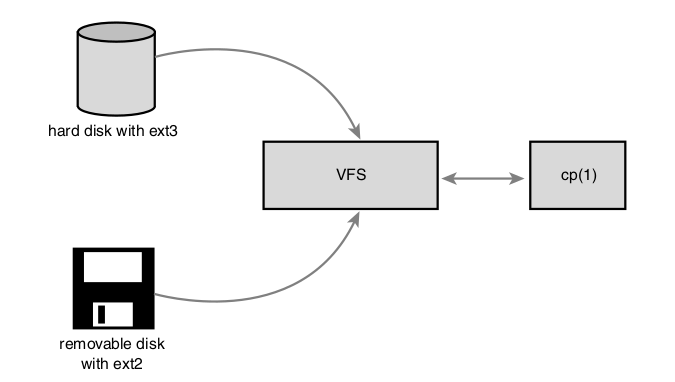
\includegraphics[width=0.7\textwidth]{ImagenesApunte/vfs.png}
\end{figure}

Cualquier cosa que vaya a ser persistida va a pasar por el VFS. Actúa como proxy, para que el kernel pueda hablar con todos. (No todos los OS tienen un VFS)

\subsubsection*{File System Abstraction Layer}
Es una interfaz genérica que para cualquier tipo de filesystem el kernel implementa con el sistema de archivos de bajo nivel. Esta capa de abstracción habilita a Linux a soportar sistemas de archivos diferentes, incluso si difieren en características y comportamiento. Esto es posible porque VFS provee un modelo común de archivos que pueda representar cualquier característica y comportamiento general de cualquier sistema de archivos.

Esta capa de abstracción trabaja mediante la definición de interfaces conceptualmente básicas y de estructuras que cualquier sistema de archivos soporta, por lo que cada filesystem adapta su forma de trabajo a lo que espera el VFS (por lo que todos los sistemas aceptan nociones como archivos, directorios, y diferentes operaciones). El resultado es una capa de abstracción general que le permite al kernel manejar muchos tipos de sistemas de archivos de forma fácil y limpia.

Establece la linea base a cumplir, después la implementación puede variar dependiendo de cada sistema.

\subsubsection*{Estructuras}
VFS tiene estructuras que modelan un file system.
\begin{itemize}
    \item Super bloque: representa a todo un sistema de archivos.
    \item Inodo (inode): representa un determinado archivo dentro de un sistema de archivos. (físico en disco)
    \item Dentry: representa una entrada de directorio, que es un componente simple de un path. (sucesión del path hasta llegar al archivo)
    \item File: representa un archivo asociado a un determinado proceso. (el proceso abrió un archivo)
\end{itemize}

\begin{figure}[!htb]
    \centering
    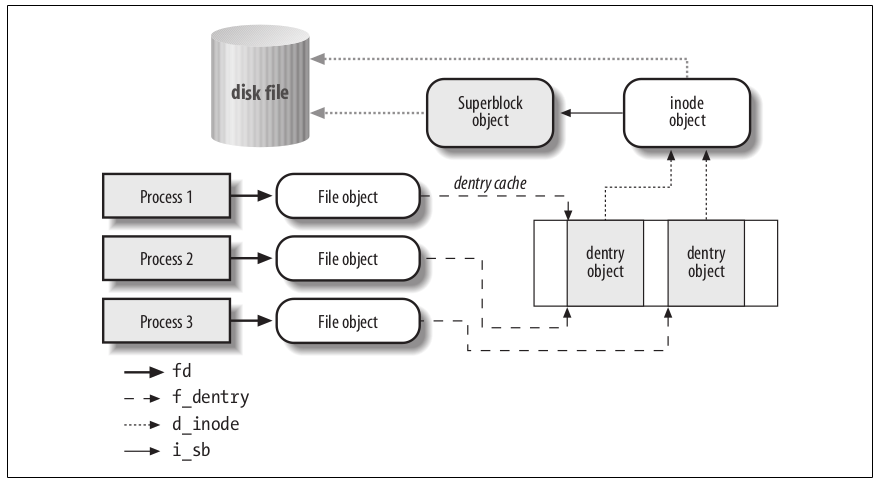
\includegraphics[width=0.8\textwidth]{ImagenesApunte/vfs_components.png}
    \caption{Notar las relaciones.}
\end{figure}

Tener en cuenta que un directorio es tratado como un archivo normal, no hay un objeto especifico para directorios. En unix los directorios son archivos normales que listan los archivos contenidos en ellos. Guardan la relación nombre del archivo-inodo. (Indica que archivos contiene el directorio)

Abrir un directorio seria ver un archivo binario, que tiene 4 bytes para ver el inodo, la longitud del archivo, la longitud del nombre, el tipo de archivo, y el nombre. (Todos tienen un '.' y '..' para representar al actual y al padre.)


\subsubsection*{Operaciones}
\begin{itemize}
    \item super\_operations: Son métodos que aplica el kernel sobre un determinado sistema de archivos. \textit{Ej. write\_inode() o sync\_fs()}.
    \item inode\_operations: Son métodos que aplica el kernel sobre un archivo determinado. \textit{Ej. create() o link()}.
    \item dentry\_operations: Son métodos que se aplican directamente por el kernel a una determinada \emph{directory entry}. \textit{Ej. d\_compare() o d\_delete(), compara elimina directorios}.
    \item file\_operations: Son métodos que aplica el kernel sobre un archivo abierto por un proceso. \textit{Ej. read() o write(), las de archivos e siempre}.
\end{itemize}

\subsection*{Archivos}

Un archivo es una colección de datos con un nombre específico. 

\textit{Ej. /home/mariano/MisDatos.txt}, cada archivo tiene un nombre único y un significado para referirse a datos. Estos nombres proveen la abstracción de mas alto nivel del dispositivo de almacenamiento. Es mas fácil manejar el nombre que el bloque en que esta guardado en disco.

Cada archivo esta dividido en 2 partes, la metadata que contiene información acerca del archivo \textit{(Ej. tamaño, fecha de modificación, propietario, seguridad)} guardada en la región conocida como \textbf{inodo}, y los datos que quieren ser almacenados (desde el OS es un arreglo de bytes sin tipo) guardados en un \textbf{data region}.

\subsection*{Directorios}
Los directorios proveen los nombres para los archivos, es una lista de nombres \emph{human-friendly} y un mapeo a un archivo o a otro directorio.

%imagenes

Definiciones:
\begin{itemize}
    \item path: es el string que identifica unívocamente a un directorio o archivo dentro de un dispositivo.
    \item root directory: es el directorio de que cuelgan todos los demás. (la raíz)
    \item absolute path: es la ruta desde el directorio raiz. \textit{Ej. home/hola/hola2}
    \item relative path: es el path relativo que se interpreta desde el directorio actual.
    \item current directory: es el directorio en el cual se ejecuta el proceso.
    \item hard link: es el mapeo entre el nombre y el archivo subyacente. Si se tiene un file system que permite muchos mapeos de estos, la estructura ya no seria un árbol (cuidado con los ciclos en estos casos). (un archivo que contiene la ruta a un archivo - un inodo puede ser apuntado por un montón de nombres - los links que tiene el inodo - es una referencia)
    \item soft link: un archivo que puede ser llamado con distintos nombres. (un archivo que apunta a otro archivo, en vez de tener un archivo directamente - un delete de un soft link no borra el archivo)
    
    \item volumen: es una una abstracción que corresponde a un disco lógico. En el caso más simple un disco corresponde a un disco físico. Es una colección de recursos físicos de almacenamiento.
    \item mount point: es un punto en el cual el root de un volumen se engancha dentro de la estructura existente de otro file system. \textit{Ej. Seria la conexión que ocurre entre el disco de la computadora y el volumen de un USB, el disco de la computadora tiene directorios preparados para realizar la unión de directorios.}
    
\end{itemize}

\textit{Cuando los links hacia un archivo llegan a 0, se borra el archivo.}

    \begin{figure}[!htb]
    \centering
    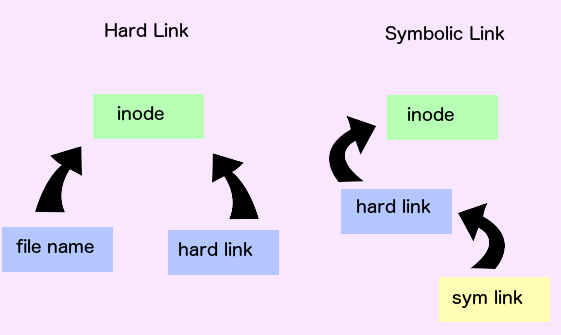
\includegraphics[width=0.7\textwidth]{ImagenesApunte/HardSoftLink.png}
    \caption{Hard y Soft Link.}
    \end{figure}
    
    \begin{figure}[!htb]
    \centering
    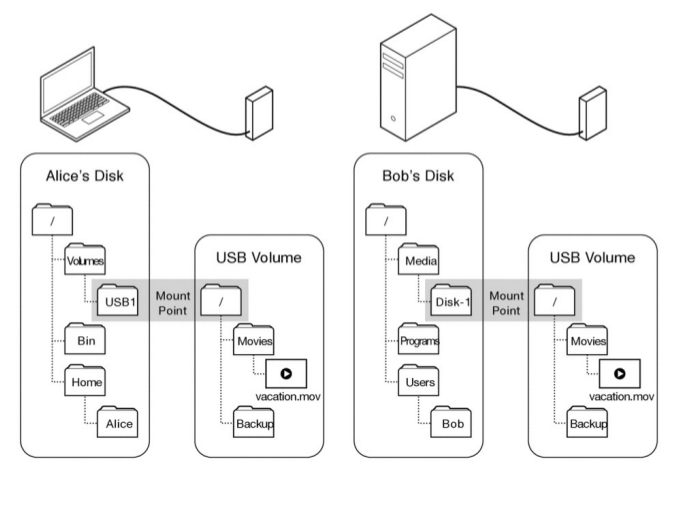
\includegraphics[width=0.7\textwidth]{ImagenesApunte/mount_point.jpg}
    \caption{Mount Point}
    \end{figure}

    \newpage


\subsection*{La API}
Varias de las mencionadas en esta lista son utilizadas en una de las tareas del lab Fork (find).

Sobre los archivos se tienen las siguientes llamadas:
\begin{itemize}
    \item open(): devuelve un file descriptor
    \item creat(): equivale a open() con unos flags en especifico, es para crear un archivo.
    \item close()
    \item read(): no garantiza la lectura total de los bytes, hace intentos de lectura.
    \item write()
    \item lseek(): reposiciona el desplazamiento de un archivo abierto.
    \item dup(): duplica el file descriptor.
    \item link(): crea un nuevo nombre para un archivo.
    \item unlink(): decrementa el contador de links sobre un inodo.
\end{itemize}

Sobre los directorios:
\begin{itemize}
    \item mkdir()
    \item rmdir()
    \item chdir()
\end{itemize}

Para trabajar sobre los directorios, incluyendo \emph{dirent.h}
\begin{itemize}
    \item opendir()
    \item readdir()
    \item closedir()
\end{itemize}

Sobre los metadatos:
\begin{itemize}
    \item stat(): devuelve información sobre un archivo.
    \item access(): determina si un proceso tiene permisos para acceder a un archivo.
    \item chmod(): altera los modos de acceso.
    \item chown(): cambia el id del propietario y el grupo de un archivo.
    \item umask(): setea una marcara con el modo de permisos para la creación de archivos.
\end{itemize}

Desde unix se tienen algunos comandos que de fondo llaman a estas syscalls.

\begin{table}[]
\centering
\begin{tabular}{|l|l|}
\hline
\multicolumn{1}{|c|}{Command} & \multicolumn{1}{c|}{System Call} \\ \hline
cat                           & read() write() open() close()    \\ \hline
rm                            & unlink() stat()                  \\ \hline
fstat                         & stat()                           \\ \hline
tee                           & open() close() read() write()    \\ \hline
touch                         & creat() stat()                   \\ \hline
ls                            & readir() write()                 \\ \hline
\end{tabular}
\end{table}

\newpage

Ejemplo de ls.
\begin{minted}{C}
    #include <stdio.h>
    #include <sys/types.h>
    #include <dirent.h>
    
    int
    main (void)
    {
        DIR *dp;
        struct dirent *ep;
    
        dp = opendir ("./");
        if (dp != NULL)
        {
            while (ep = readdir (dp))
                puts (ep->d_name);
            (void) closedir (dp);
        }
        else
            perror ("Couldn't open the directory");
    
        return 0;
    }
\end{minted}

Ejemplo de Copy.

\begin{minted}{C}
    #include <stdio.h>
    #include <unistd.h>
    #include <sys/types.h>
    #include <sys/stat.h>
    #include <fcntl.h>
  
    int
    main(int argc, char *argv[])
    {
        int fdold, fdnew;
        if (argc!=3){
           fprintf(stderr, "Se precisan 2 argumentos\n");
           exit(1);
        }
        fdold=open(argv[1], O_RDONLY);
        
        if (fdold==-1){
                   fprintf(stderr, "No se pudo abrir el fichero %s\n",
                   argv[1]);
                   exit(1);
        }
        
        fdnew=creat(argv[2], 0666);

        if (fdnew==-1){
               fprintf(stderr, "No se pudo crear el fichero %s\n",
               argv[2]);
               exit(1);
        }

        copy(fdold, fdnew);
        exit(0);
    }
    
    void 
    copy(int old, int new)
    {
         int cuenta;
         char buffer[2048];

        while ((cuenta=read(old, buffer, sizeof(buffer)))>0)
            write(new, buffer, cuenta);
    }
\end{minted}

\subsection*{Implementación}

Se ve un vsfs (very simple file system)

\begin{itemize}
    \item Se necesita una estructura de datos de un sistema de archivos, la forma de guardar la información en el disco (los datos y metadatos). Este sistema usa un arreglo de bloques.
    \item Se define un método de acceso, como relacionar las llamadas de los procesos al sistema de archivos (\textit{open(), read(), ...})
\end{itemize}

Son N bloques de 4kb. La mayor parte del espacio utilizado va a ser para la data region. Estas regiones tienen sus metadatos, los cuales se guardan en inodos, que deben guardarse a disco también en una inode table (arreglo de inodos almacenados en disco). Los inodos no son estructuras grandes (128,256 bytes). Los inodos representan la cantidad máxima de archivos que podrá contener el sistema de archivos también.

Otra cosa que hay que saber, es que inodos y bloques están siendo utilizados (o están libres), la estructura encargada de esto se llama estructura de alocación. En esta implementación se utiliza un bitmap, una para los datos (data bitmap) y otra para los inodos (inode bitmap). En esta estructura se mapea un 0 si esta libre, y un 1 si esta ocupada. Cada bitmap ocupa menos de 4kb, pero se utiliza un bloque por cada uno. (un bloque para inodos y otro bloque para datos)

También esta el Super Bloque (S), que contiene la información de todo el file system. Esto es, la cantidad de inodos, de bloques, donde comienza la tabla de inodos, donde están los bitmaps.

Se muestra un ejemplo de 64 bloques de 4kb, 56 bloques son para datos. Cada bloque de 4kb puede guardar 16 inodos (suponiendo que ocupan 256 bytes), se tienen 5 bloques de inodos (80 inodos). Un bloque para cada bitmap (I) (D), y el super bloque (S)

    \begin{figure}[!htb]
    \centering
    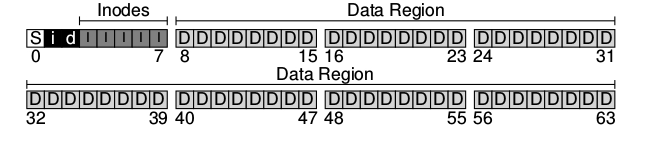
\includegraphics[width=0.7\textwidth]{ImagenesApunte/distribucionDisco.jpg}
    \caption{Distribución del ejemplo.}
    \end{figure}

\subsubsection*{Inodos}
Se refiere a un inodo a través de un inumber, dado un inumber se puede saber directamente en que parte del disco se encuentra el inodo.

Para leer el inodo numero 32, el sistema de archivos debe: 
\begin{enumerate}
    \item debe calcular el offset en la regio de inodos 32* sizeof(inode) = 8192.
    \item sumarlo a la dirección inicial de la inode table en el disco o sea 12Kb+ 8192 bytes.
    \item llegar a la dirección en el disco deseada que es la 20 KB.
\end{enumerate}

    \begin{figure}[!htb]
    \centering
    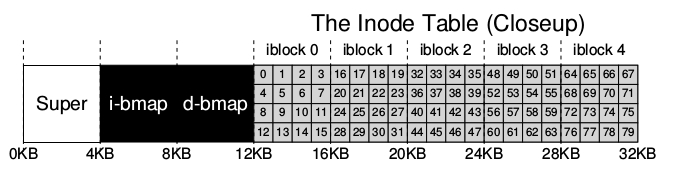
\includegraphics[width=0.7\textwidth]{ImagenesApunte/inodes.jpg}
    \end{figure}
    
    \begin{figure}[!htb]
    \centering
    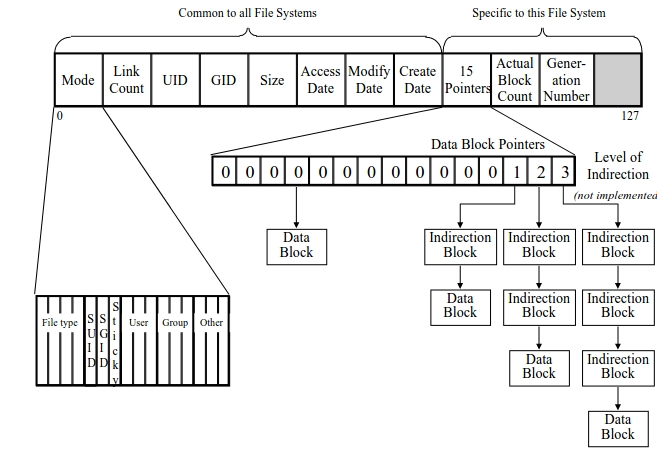
\includegraphics[width=0.7\textwidth]{ImagenesApunte/inode.jpg}
    \end{figure}

\newpage

% volver a correr pruebas tp3 antes 
% interfaces al conectar dispositivos: IDE/ATA (disco optico) - NVMe (disco estado solido) - qemu emula un disco de tipo ide - jos accede con in y out, no pasa por memoria mapeada
% esquemas (de interaccion): polling (ctemente pullea)vs interrupciones - PIO (cpu accede a disco directamente) vs DMA (direct memory access)(el cpu delega a otra parte del hardware) 
% jos usa polling
% bloque y sector son unidaes de memoria, un sector es la unidad minima en la que opera el hardware, el SO lo abstrae en bloques (multiplo del tamaño de un sector)
% en jos los sectores son de 512B, los bloques de 4096B (mismo que una pagina) - siempre se le dice que lea y escriba en sectores al disco, el driver del disco sabe como convertir bloques en sectores y al reves.
%
% bloque 0 mbr y//o tabla de particiones - esta el bootloader (master boot loader o tabla para uefi)
% bloque 1 es el superbloque - informacion del filesystem
% subsistemas implementados desde el lado del usuario
% el struct file es un inodo y una directory entry a la vez (los directorios funcionan como inodos) 
% qemu emula 2 discos - el 0 usado solo para el boot, el disco 1 usa una imagen separada, jos implementa un controlador IDE sin interrupciones
%
% VFS - interfaz entre cualquier implementacion de filesystem y userspace - se puede delegar al usuario FUSE
% jos no tiene syscall de acceso a disco, no hay VFS - existe un proceso con privilegios especiales que maneja el acceso a disco (envfs - tipo especial de environment) - se comunica con el con envfs, envfs accede directamente a disco
% mappear on demand, reservo algo, y si alguien la pide la mappeo
% CACHE DE BLOQES se mantiene un mapeo lazy de todo el disco en memoria - 1 pagina = 1 bloque - tiene su propio pgfault_handler - maximo 3gb
% lazy, dejo todo mapeado, y cuando alguien quiera acceder lo traigo de disco
% aprovechar PTE_D para saber si hubo modificaciones, las paginas quedan mapeadas por siempre (esta siempre sincronizada con lo que haya en disco, salvo cuando haya flush (tiempo muy corto))
% BITMAP compacto, cada bit es un bloque - algun bloque del disco es el bitmap, indica que bloques estan libres
% interpretar como un entero, y realizar shift, realizando operaciones de bits
% envfs se queda loopeando escuchando requests
% las estruccturas las maneja la biblioteca de jos
% cada proceso recibe una referencia a ese archivo abierto y lo guarda en una tabla de file descriptors
% el proceso de usuario use el indice en su tabla, pero usa el ID de envfs para hacer requests
%
%%%%%%%%%%%%%%%%%%%%%%% TP 4
% fs - file system, el codigo del proceso encargado de mantenerlo
% ide.c funciones de bajo nivel que leen y escriben de disco - usa inb y outb - espera a que el disco responda - usamos ide_read e ide_write - a partir de un sector (secno), tantos sectores (nsecs) a escribir/leer- direccion para los datos (src/dst)
% va_is_dirty(...) para saber si esta dirty
% inicializar el bc es configurar el pg_fault_handelr - (no carga nada a disco hasta que se accede al disco) - hay funcionas para preguntar si un bloque esta libre
% block_alloc - recorrer el bitmap hasta encontrar 1

% struct File* es un puntero a un'inodo', devolver en la variable ** un puntero al numero que contiene al bloque (filke_block_walk) similar a pgdir_walk pero para inodos y files - encuentra el slot, no el bloque, EL SLOT! la direccion de memoria de donde esta guardada
% file_get_block() equivale a pg_lookup(), devuelve el numero de bloque
% serve while eterno - ipc_recv
% maximo 32 FD en la tabla - hay 3 tipos de dispositivos inc/fd.h
% struct Dev -  establece una 'herencia' de funciones, cada sistema debe de soportarlas
%
% SIEMPRE QUE SE MODIFIQUE UN BITMAP HACER UN FLUSH
% 
% spawn -> es hacer una especie de load_icode en modo usuario
% mini syscall para cambiar el eip - jos valida que sea padre y el eip sea valido
% va armando el trapframe
% llama a sys_env_set_trapframe, con esto lo setea
%
% init_stack, complicado de hacer porque hay que prepararlo para que tenga los argumentos que recibe, en linux lo setea exec, en jos lo hace el init_stack - cuenta argumentos, calcula memoria y lo configura
% sys_env_trapframe, permite modificar desde el user space - revisar varias condiciones
% si tenemos funcion spawn, podemos realizar una shell, nos viene una mini-shell
% pagina de fd que no se replique bajo ninguna circunstancia - se agrega un flag - PTE_SHARE - le indica a fork que ciertos mapeos de pagina es compartida, que no haga COW
% ya ciertas partes del codigo usan el flag
% kbd_interrupt - toda la entrada por teclado hasta ahora nunca fue al monitor
% shell, agregar una funcion de redireccion usando el filesystem de jos
% console.c
% mucho codigo que no se toca, revisarlo
% lo importante es entender como funciona el filesystem y el environment (0 a 3)

\section{Extras}
\subsection*{Octava clase}
\subsection{Shell scripting}
Algunas notas de shell scripting, se da como extra en la virtualidad. Información completa en el
\href{https://www.gnu.org/savannah-checkouts/gnu/bash/manual/bash.html}{manual}.

Para hacer un script normalmente se dice que interprete o shell script se va a usar.
Se empieza con \#!/bin/bash por ejemplo
\subsubsection*{Built in}
Comandos que ejecuta la propia shell, sin la necesidad de crear un nuevo proceso. \textit{Los siguientes fueron implementados en el lab shell.}
\begin{itemize}
    \item echo
    \item cd
    \item pwd
    \item ...
\end{itemize}

\subsubsection*{Variables}
En las shell se pueden definir variables. Todas son de tipo string, para otro caso hay que definirlo especificamente.
\begin{minted}{bash}
      NOMBRE = "nombre"
\end{minted}

Se obtiene el valor con el \$:
\begin{minted}{bash}
    $ echo $NOMBRE
    nombre
\end{minted}

\subsubsection*{Variables magicas}
Hay un monton de variables propias de la shell, algunos ejemplos son:
\begin{itemize}
    \item \$? : Tiene el resultado del ultimo programa ejecutado.
    \item \$\# : Tiene el numero de argumentos.
    \item ...
\end{itemize}

\subsubsection*{Arreglos}
\begin{minted}{bash}
    array = (1 2 3 4 5)
\end{minted}

Para verlo:
\begin{minted}{bash}
    echo array
    echo ${array[3]}
\end{minted}

\subsubsection*{Estructuras de control}
Hay diferentes estructuras de control. Se pueden comparar valores numericos y strings, usar if, y loops.

\subsubsection*{Funciones}
A diferencia de las funciones de los lenguajes de programación 'reales', las funciones Bash no pueden devolver un valor cuando se las llama. Cuando se completa una función bash, su valor de retorno es el estado de la última instrucción ejecutada en la función, 0 para el éxito y un número decimal distinto de cero en el rango de 1 a 255 para el fracaso.

El estado de retorno puede especificarse utilizando la palabra clave return y se asigna a la variable \$?. La utilización de return termina la función.

\subsection*{Charla}
\subsection{Internals de Git}

Git hace varias cosas, una de ellas es el control de versiones. ¿Como hace para ir viendo la evolución del archivo? ¿Como se implementaría?
Viéndolo con un ejemplo, tengo un único archivo (fisop.txt) y le hacemos un único cambio. Quiero mantener el estado histórico en los tiempos T1 y T2. Hay dos estrategias para guardarlas, una es guardar una copia del archivo entero, otra es guardar la diferencia, no todo el archivo.

Guardando solo la información nueva, se tiene una estrategia mas eficiente en espacio, pero es poco eficiente en la recuperación de estados anteriores, hay que ir reconstruyendo el archivo.

La otra alternativa de guardar las copias del archivo, es mas rápido en mostrar las versiones (no hay que reconstruir desde el comienzo), pero es poco eficiente en el uso de espacio.

Git usa ambas opciones, pero principalmente usa la versión de Snapshots (copias de todos los archivos enteros en todos los momentos). La historia no se puede cambiar, pero si se puede reescribir (esta todo referenciado). Git nunca guarda el mismo contenido mas de una vez, se da cuenta git que lo tenia guardado. De esta forma contra resta la parte mala del uso de Snapshots.

\subsubsection*{blob}
Git se maneja con objetos, necesitamos una forma de modelar los archivos y sus contenidos. Objeto de tipo \textbf{blob}, representa los contenidos totales de un archivo. Si se cambia un archivo, se crea un blob nuevo. Todo blob tiene un nombre (no el del archivo), se obtiene con un hash (cadenas hexadecimales). \textit{Ej. 23fca84...}. 

\begin{itemize}
    \item git cat-file [-p|-t] <shasum> : Muestra contenido/tipo de un objeto, <shasum> es un hash
    \item git ls-files --stage : Muestra los archivos index y working directory
\end{itemize}

Si todos tenemos el mismo contenido, vamos a tener el mismo nombre de blob.

Los blob no pueden representar directorios.

\subsubsection*{tree}
Los directorios se modelan como objeto \textbf{tree}. Contiene referencias a otros trees y blocs. Le da nombre a archivos y directorios. Todo tree tiene un nombre (no el del directorio) que se obtiene de un hash también.

\begin{itemize}
    \item git diff-tree <tree-ish> <tree-ish> : Compara dos trees y los contenidos de sus blobs
    \item git ls-tree : Muestra los contenidos de un tree
\end{itemize}

\subsubsection*{commit}
Representa un snapshot del repositorio que contiene referencias a un único tree, metadata del snapshot (autos, cuando se hizo), uno o mas padres, y un nombre (no el del snapshot).

Si el archivo no cambia, los blobs se reutilizan. (No importa que nombre tenga el archivo, solo importan los contenidos)

\subsubsection*{tag}
Representa una referencia a un objeto. Contiene referencias a un único objeto, metadata (autor, nombre, mensaje), y un nombre (no el del tag).

No todos los tags son objetos, solamente los \textbf{annotated tags}.

\subsubsection*{¿Como se guardan?}
Git mantiene un mapa de objetos dentro de \emph{.git/objects}. Cada objeto tiene como nombre su hash. Se guardan en shards para accederlos de forma mas eficiente. (Primeros 2 dígitos como nombre de una 'carpeta').

\subsubsection*{Ramas}
No son objetos, toda branch es una referencia a un commit. Se guardan en \emph{.git/refs}. HEAD es una referencia a una branch.

\subsubsection*{Packing objects y pruning}
Guarda archivos enteros, no usa deltas, pero permite empaquetar objetos.

Compacta objetos en un único archivo guardándolos como diff a otro objeto.

Es eficiente para almacenar y transferir repositorios grandes.

\begin{itemize}
    \item git prune: elimina objetos que no son alcanzables de la base de datos de git
    \item git count-objets: Cuenta la cantidad de objetos que se tienen y muestra cuanto pesa el repositorio
    \item git pack-objects: Crea manualmente un empaquetamiento de objetos
\end{itemize}

Si se crea un archivo muy grande y se borra, sigue referenciado, por lo que el repositorio va a seguir pesando eso. Por eso es malo subir imágenes/vídeos grandes a git si no son realmente necesarios.







\newpage


\section{Bibliografía}\label{sec:bibliografia}
La bibliografía utilizada en la materia es la siguiente:
\begin{itemize}
    \item Operating Systems: Principles and Practice - Thomas Anderson y Michael Dahlin
    \item Operating Systems: Three Easy Pieces - Remzi H, Arpaci-Dusseau y Andrea C. Arpaci-Dusseau\footnote{Gratuito desde \href{http://ostep.org/}{http://ostep.org/}}
    \item UNIX Internals: The New Frontiers - Vahalia, Uresh. Pearson Education India
    \item Computer Systems: A Programmer’s Perspective - Randal E. Bryant, David R. O’Hallaron, Prentice Hall
    \item The Design of the UNIX Operating System - Bach, Maurice J. Prentice-Hall
    \item The Linux Programming Interface - Michael Kerrisk
\end{itemize}



\end{document}










